\chapter{Scheduling with Oracles}
\label{ch:oracle}

\begin{abstract}
A classic problem in parallel computing is determining whether to
execute a task in parallel or sequentially. If small tasks are
executed in parallel, the task-creation overheads can be overwhelming.
If large tasks are executed sequentially, processors may spin
idle. This granularity problem, however well known, is not well
understood: broadly applicable solutions remain elusive.  

We propose techniques for controlling granularity in implicitly
parallel programming languages.  Using a cost semantics for a
general-purpose language in the style of the lambda calculus with
support for parallelism, we show that task-creation overheads can
indeed slow down parallel execution by a multiplicative factor.  We
then propose {\em oracle scheduling}, a technique for reducing these
overheads, which bases granularity decisions on estimates of
task-execution times.  We prove that, for a class of computations,
oracle scheduling can reduce task creation overheads to a small
fraction of the work without adversely affecting available
parallelism, thereby leading to efficient parallel executions.

We realize oracle scheduling in practice by a combination of static
and dynamic techniques.  We require the programmer to provide the
asymptotic complexity of every function and use run-time profiling to
determine the implicit, architecture-specific constant factors. In our
experiments, we were able to reduce overheads of parallelism down to
between 3 and 13 percent, while achieving 6- to 10-fold speedups.


%% We realize the oracle scheduling in practice by combining static and
%% dynamic techniques. We require the programmer to provide asymptotic
%% complexity functions for parallel tasks and use run-time profiling to
%% determine hardware-specific constant factors.  We implement the
%% proposed approach by extending the Manticore compiler for Parallel ML.
%% Consistent with our theoretical results, experiments show that oracle
%% scheduling can reduce the task-creation overheads down to between 3
%% and 13 percent of the sequential time and yield scalable speedups
%% when running on multiple processors.

%old paragraph
%To realize oracle scheduling in practice, we develop an approach based
%on an seemingly unlikely insight: asymptotic complexity of parallel
%task can be used estimate their actual run-times by judicious use of
%profiling.  We propose language constructs for annotating parallel
%tasks with their asymptotic complexity and propose techniques for
%compiling these programs into efficient parallel executables.  We
%prove the compilation technique correct and implement it by extending
%the Manticore compiler and the run-time system to support oracle
%scheduling and perform an evaluation.  Our experiments show that the
%approach can improve overheads show...  \uremark{Imp and Exp, check.}


%Our results include analytical bounds, programming-language constructs
%for guiding task-creation, and techniques for compiling programs
%annotated with these constructs into efficient parallel executables,
%and an implementation.

\end{abstract}




% TO CHANGE  
\category{D.1.3}{Programming Techniques}{Concurrent Programming}
%\subjects{Parallel Programming}
\terms{Algorithms, Experimentation, Languages}
\keywords{Scheduling, Granularity Control, Work Stealing}



\begin{comment}
\begin{abstract}

A classic problem in parallel computing is determining whether to
execute a task in parallel or sequentially. If many small tasks are
executed in parallel, the overhead of creating these parallel tasks
can be overwhelming.
If many large tasks are executed
sequentially, processors may spin idle, resulting again in suboptimal
speedups. Although identified as an important problem with practical
importance, the theoretical underpinnings of this problem are not well
understood and broadly applicable solutions are lacking.

In this paper, we propose techniques for controlling the scheduling
overheads of task creation to achieve parallel efficiency.
Specifically, we extent Brent's theorem~\cite{Brent74} (a.k.a.'s
work-time principle) to include task creation overheads.  Using a cost
semantics for a general-purpose language in the style of lambda
calculus with parallel tuples, we then show that task-creation
overheads can slowdown parallel execution by a multiplicative factor.
To reduce the overheads, we introduce {\em oracle scheduling}, a
semantics guided by estimates of the sizes of parallel tasks.  We show
that if the oracle provides in constant time estimates that are
accurate within a constant multiplicative factor then oracle
scheduling provable reduces the task-creation overheads for a broad
range of parallel computations.




%% We realize oracle scheduling in practice by a combination of static
%% and dynamic techniques.  We require the programmer to provide the
%% asymptotic complexity of every function and use run-time profiling to
%% determine the implicit, architecture-specific constant factors. We
%% have experimented our oracle scheduling approach by extending the
%% Manticore compiler. Using the approach, we were able to reduce the
%% overheads of the total sequential execution time, down to between 3
%% and 13 percent.  When using 16 processors, we achieved 7- to 15-fold
%% speedups on an AMD machine and 6- to 10-fold speedups on an Intel
%% machine.


%% To realize oracle scheduling in practice, we rely on a combination of
%% static and dynamic techniques.  We require the programmer to provide
%% the asymptotic complexity of every function and use this information
%% at compile time to instrument the source code.  We then use run-time
%% profiling to determine the constant factors that applies to every
%% complexity expression. We have experimented our oracle scheduling
%% approach by extending the Manticore compiler. We were able to reduce
%% the overheads of the total sequential execution time, down to between
%% 3 and 13 percent.  When using 16 processors, we achieved 7- to 15-fold
%% speedups on an AMD machine and 6- to 10-fold speedups on an Intel
%% machine.

%old paragraph
%To realize oracle scheduling in practice, we develop an approach based
%on an seemingly unlikely insight: asymptotic complexity of parallel
%task can be used estimate their actual run-times by judicious use of
%profiling.  We propose language constructs for annotating parallel
%tasks with their asymptotic complexity and propose techniques for
%compiling these programs into efficient parallel executables.  We
%prove the compilation technique correct and implement it by extending
%the Manticore compiler and the run-time system to support oracle
%scheduling and perform an evaluation.  Our experiments show that the
%approach can improve overheads show...  \uremark{Imp and Exp, check.}


%Our results include analytical bounds, programming-language constructs
%for guiding task-creation, and techniques for compiling programs
%annotated with these constructs into efficient parallel executables,
%and an implementation.

\end{abstract}
\end{comment}


\section{Introduction}
\label{sec:introduction}

%-----------------------
%\paragraph{Motivation}
{\em Explicit parallel programming} provides full control over
parallel resources by offering primitives for creating and managing
parallel tasks, which are small, independent threads of control.   % ARTHUR: FIX THIS
As a result, the programmer can, at least in principle, write efficient
parallel programs by performing a careful cost-benefit analysis to
determine which tasks should be executed in parallel and under what
conditions.  This approach, however, often requires reasoning about
low-level execution details, such as data races or concurrent effects,
which is known to be notoriously hard; it can also result in code that
performs well in a particular hardware setting but not in others.

The complexities of parallel programming with explicit languages have
motivated interest in {\em implicitly parallel languages}, such as
Cilk~\cite{Blumofe95},
Manticore~\cite{Fluet:2008:SFG:1411204.1411239,FluetRaReSh11},
Multilisp~\cite{Halstead85}, and NESL~\cite{nesl-implement}.  These
languages enable the programmer to express opportunities for
parallelism via language constructs, \textit{e.g.}, parallel
sequences, parallel arrays, and parallel tuples.  This implicit
approach enables a declarative programming style by delegating the
task of utilizing the parallelism exposed by the program to the
compiler and the run-time system.  As an implicit parallel program
executes, it exposes opportunities for parallelism (as indicated by
the parallel constructs) and the language run-time system creates
parallel tasks as needed.  To execute parallel tasks efficiently,
implicit programming languages use a scheduler to load balance,
\textit{i.e.}, distribute parallel tasks among processors.  Various
scheduling techniques and practical schedulers have been developed,
including work-stealing
schedulers~\cite{BlumofeWorkStealing,AroraBlPl98,AcarBlBl02} and
depth-first-search schedulers~\cite{BlellochGr96}.

Experience with implicitly parallel programs shows that one of the
most important decisions that any implicit parallel language must make
is determining whether or not to exploit an opportunity for
parallelism by creating a parallel task.  Put another way, the
question is to determine which tasks to execute in parallel and which
tasks to execute sequentially.  This problem, often referred to as the
{\em granularity problem}, is important because creating a parallel
task requires additional overhead. If the task granularity is not
handled effectively, task-creation overheads can easily obliterate the
benefit of parallelism.

%% Because the speedup achievable
%% via parallel computation is bounded by the number of processors, often
%% a small constant factor, any increase in the overhead, however small,
%% matters.

Many parallel programs are characterized by parallel
slackness~\cite{Valiant90}, a property which indicates that the
program exposes many more opportunities for parallelism than the
number of available processors. In such programs, effective
granularity control is crucial because the program typically creates
many small tasks, thereby ensuring significant scheduling overhead.

% (a.k.a., parallel slackness~\cite{Valiant90})

No known broadly applicable solution to the granularity problem
exists. Theoretical analyses often ignore task-creation overheads,
yielding no significant clues about how these overheads may affect
efficiency.  Practical implementations often focus on reducing
task-creation overheads instead of attempting to control granularity.
As a result, practitioners often deal with this issue by trying to
estimate the right granularity of work that would be sufficiently
large to execute in parallel.  
% umut: this seems redundant. also wrong use of ``to pay off'' 
% More specifically, programmers try to determine the input sizes at
% which tasks become too small to pay off the costs of parallel task
% creation and sequentialize such tasks.
%
Since the running time of a task depends on the hardware, such manual
control of granularity is difficult
and bound to yield suboptimal results and/or non-portable
code~\cite{lazy-binary-splitting}.

% umut:reformulated this.
% the programmer must make the best decision they can by taking into
% account the specifics of the hardware.  This manual granularity
% control is bound to yield suboptimal results and/or non-portable
% code~\cite{lazy-binary-splitting}.

%There is some recent work on the area of performance tuning of benchmarks
%by profiling certain specific
%parameters~\cite{performance-tuning}.

In this paper, we propose theoretical and practical techniques for the
granularity problem in implicit parallel-programming languages.  Our
results include theorems that characterize how parallel run time is
affected by task-creation overheads, which we show to be significant
(\secref{theorems}).  To reduce these overheads, we consider
a granularity control technique that relies on an oracle for
determining the run-time of parallel tasks (\secref{cost-semantics}).  We
show that if the oracle can be implemented efficiently and accurately,
it can be used to improve efficiency for a relatively large class of
computations (\secref{theorems}). 
Based on this result, we describe how oracles can be
realized in practice; we call this technique {\em oracle scheduling}
because it relies on an oracle to estimate task sizes and because it
can be used in conjunction with practically any other scheduler
(\secref{schedule}).  Finally, we propose an implementation of oracle
scheduling that uses complexity functions defined by the user to
approximate accurately run-time of parallel tasks (\secref{schedule}).
We present an implementation and evaluation of the proposed approach
by extending a subset of the Caml language (\secreftwo{imp}{exp}).

Brent's theorem~\cite{Brent74}, commonly called the work-time
principle, characterizes what is arguably the most important benefit
of parallel programs, which is that a parallel program can be executed
on a multiprocessor to obtain near linear speedups.  For a
computation, let {\em raw work}, written $\sw{}$, refer to the total
number of executed instructions, and let {\em raw depth}, written $\sd$,
refer to the length longest dependent chain of executed instructions.
Brent's theorem shows that we can execute a computation with $\sw$ raw
work and $\sd$ raw depth in no more than $\sw/P + \sd$ steps on $P$
processors using any \emph{greedy scheduler}. (Note that the
  bound is tight within a factor of two.)  A greedy scheduler is a
scheduler that can find available work immediately.  This assumption
is reasonably realistic, as practical multiprocessor scheduling
algorithms, such as work-stealing, can match Brent's bound
asymptotically for certain relatively large classes of computations,
\textit{e.g.}, fork-join and nested data-parallel computations.

In the execution model with raw work and raw depth, each instruction
implicitly is assigned unit cost.  Unfortunately, this model does not
direcly account for task-creation overheads.  To assess the
significance of these overheads in implicitly parallel programs, we
consider a lambda calculus with parallel tuples and present a
cost-semantics for evaluating expression of this language
(\secref{cost-semantics}).  The cost semantics accounts for
task-creation overheads by assigning non-unit costs to the operations
generating such overheads.  In addition to raw work and raw depth, the
cost semantics yield total work, total depth of each evaluated
expression.  We define {\em total work}, written $\sws$, as the total
cost of the evaluated instructions, and {\em total depth}, written
$\sds$, as the total cost of the most expensive dependent chain of
evaluated instructions---total work and total depth include
task-creation overheads.

Using this cost semantics, we show that task creation overheads can be
a significant multiplicative factor of the raw work.  To understand
the understand the impact of the overheads, we adapt Brent's theorem
to take them into account (\secref{cost-semantics}).  Specifically, we
show that parallel computations with total work $\sws$ and total
depth $\sds$ can be executed in no more than $\sws/P + \sds$ steps.
Intuitively, this bound shows that task-creation overheads contribute
directly to the parallel run time just like any other work.  Combined
with the result that task-creation overheads can increase total work
by a multiplicative factor, the generalized Brent's theorem implies
that the overheads slow down parallel run time by a multiplicative
factor.

To reduce task-creation overheads, we propose an alternative {\em
  oracle semantics} that capture a well-known principle for avoiding
the task-creation overheads. We evaluate a task in parallel only if
its is sufficiently large, \textit{i.e.}, greater than some {\em
  cutoff} constant $\coff$.  We show that the oracle semantics can
decrease the overheads of task-creation by any desired constant
factor $\coff$, but only at the cost of increasing the total depth
(\secreftwo{cost-semantics}{analysis}).
%
These bounds suggest that we can reduce the
task-creation overheads significantly, if we can realize the semantics
in practice.  This  unfortunately is impossible because it requires
determining a priori task-creation overheads.  We show, however, that
a realistic oracle that can give constant-factor approximations to the
task run times can still result in similar reductions in the
overheads. We show that if we have prior knowledge of the
raw work and the raw depth of a computation, then we can pick the
optimal cutoff constant $\coff$ that yields the fastest parallel run
time for a class of computations.  We also show that, under some
assumptions, there exists a constant $\coff$ that reduces the task
creation overheads to a small constant ratio of the raw work, without
increasing the depth of the computation in a way that would 
significantly affect the run time. %ARTHUR: check this


To realize the oracle semantics in practice, we describe a scheduling
technique that we call {\em oracle scheduling} (\secref{schedule}).
Oracle scheduling relies on a {\em task-size estimator} that can
estimate the actual run time of parallel tasks in constant-time within
a constant factor of accuracy, and a conventional greedy scheduling
algorithm, \textit{e.g.}, work-stealing, or a parallel depth-first
scheduler.  Oracle schedulers perform efficient parallel task creation
by selectively executing in parallel only those tasks that have a
large parallel run-time. We describe an instance of the oracle
scheduler that relies on an estimator that uses asymptotic cost
functions (asymptotic complexity bounds) and judicious use of run-time
profiling techniques to estimate actual run-times accurately and
efficiently.  This approach combines an interesting property of
asymptotic complexity bounds, which are expressed without
hardware-dependent constants, and profiling techniques, which can be
used to determine these constants precisely.

We present a prototype implementation of the proposed approach
(\secref{imp}) by extending the OCAML language to support parallel
tuples and complexity functions.  The implementation translates
programs written in this extended language to the PML (Parallel ML)
language~\cite{FluetRaReSh11}.  Although our implementation requires
the programmer to enter the complexity information, this information
could also be inferred in some cases via static analysis
(\textit{e.g.},~\cite{JostHaLoHo10} and references therein).  In our
implementation, for simplicity we only consider programs for which the
execution time is (with high probability) proportional to the value
obtained by evaluating the asymptotic complexity expression.  We
extend the Manticore compiler for PML to support oracle scheduling and
use it to compile generated PML programs.  Our experiments
(\secref{exp}) show that oracle implementation can reduce the
overheads of a single processor parallel execution to between 3 and 13
percent of the sequential time.
When using 16 processors, we achieve 7- to 15-fold speedups
on an AMD machine and 6- to 10-fold speedups on an Intel machine.

%% %-----------------------
%% \paragraph{Realizing the oracle}
%% %
%% \aremark{The following paragraph is good but a bit too verbose I find}
%% As a practical realization of the oracle semantics, we propose in this
%% paper techniques that combine the user-provided portable annotations
%% with judicious use of run-time profiling during run-time.  The key
%% insight behind our proposal is the realization that the asymptotic
%% complexity of parallel tasks offer portable (hardware independent)
%% information about the run-time of parallel tasks and they can be used
%% to infer actual run times when combined with careful profiling.  To
%% see this, suppose that we know the asymptotic complexity of each
%% parallel task. By definition, asymptotic complexity ignores constant
%% factors and thus remains unchanged across a range of parallel systems
%% or computers. The ignored constant factors, however, 
%% are very hard to predict statically. Since those factors can be large,
%% complexity bounds themselves do not constitute good estimators
%% for the purpose of realizing the oracle semantics in practice.  Given
%% the asymptotic complexity of a task, and the actual value of the input
%% size or parameter that the complexity depends on, we can determine
%% relatively easily the constant factors hidden by the asymptotic
%% notation by taking a few samples.  Specifically, we can measure the
%% run-time of the task and using relatively straightforward curve
%% fitting techniques determine the hidden constant factor.  When a
%% similar task is then executed again (with any other input), we can
%% then estimate its size by using the determined constants and the
%% asymptotic formula.

%\paragraph{Compilation}

%\paragraph{Implementation}

%TODO: should say we do work-stealing.
% here is a short summary
%The work-stealing scheduler has been successfully used to implement parallel tuples.
%When evaluating a parallel tuple, the second branch of the tuple is placed on
%the processor's {\em deck}, rather than on the processor's stack.
%Processor that do not have work to do look at the deck of other processors
%to try and steal a task from them.
%Placing tasks on the deck is more expensive
%than placing them on the stack, and this is where the overhead is coming from


%------------------

%\paragraph{Experiments}




\begin{comment}

\section{Generalizing Brent's theorem}
\label{sec:brent}
%{Work-Time Principle with Scheduling Overheads}

\begin{figure}
\centering
\ifx\arthur\false
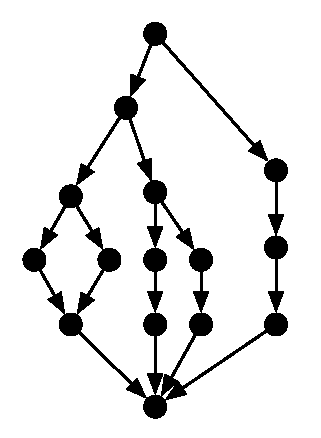
\includegraphics[width=0.4\columnwidth]{pictures/computation-dag}
\fi
\caption{An example computation DAG.}
\label{fig:dag}
\end{figure}


%\subsection{Computation Dags}


We represent a parallel computation with a directed acyclic graph, 
called {\em computation DAG}. Nodes in the graph represent
atomic computations.
Edges between nodes represent precedence relations,
in the sense that an edge from $a$ to $b$ indicates that the execution of $a$ must
be completed before the execution of $b$ can start.
Every computation DAG includes a {\em source} node and a {\em sink} node,
representing the starting and the end points of the computation, respectively.  
Those nodes are such that all nodes of a computation DAG are reachable from
the source node, and the sink node is reachable from all nodes.
An example computation DAG appears in \figref{dag}.

In the traditional computational model, every atomic computation is
considered to take a single unit of time. In other words, every
node has weight $1$. In this setting, we can
define the standard notion of work and depth, which we here
call {\em raw work} and {\em raw depth}.
The {\em raw work} of a computation graph is equal to the total number of 
nodes that it contains. The {\em raw depth} of the computation graph
is equal to the total number of nodes along the longest path.
Brent proved the following bound.

\begin{theorem}[Brent's theorem]
\label{lem:brent}
Let $G$ be a computation DAG with $\sw$ raw work and $\sd$ raw depth.
Any greedy scheduler can execute the computation in $G$ 
in time $O(\frac{\sw}{P} + d)$ on a $P$-processor parallel machine
\end{theorem}
\begin{proof}
We recall Brent's proof since our aim is to generalize it.
Consider the nodes at depth $i$ in the DAG, and assume there are
$\sw_i$ of them. A greedy scheduler can spend no more than time
$\ceil{\frac{\sw_i}{P}}$ for executing those nodes. 
Summing up over the various depths, one can thus deduce that
the total execution time does not exceed:
$$\sum_{i=1}^{\sd}{\ceil{\frac{\sw_i}{P}}}
\Sc\leq \sum_{i=1}^{\sd}{(\frac{\sw_i}{P}+1)}
\Sc\leq \frac{\sum_{i=1}^{\sd}{\sw_i}}{P} + \sd
\Sc\leq \frac{\sw}{p} + \sd$$
\qed
\end{proof}
Observe that the bound provided by Brent's theorem is tight,
because the execution time is at least $\kwmax{ \frac{\sw}{P} }{ \sd }$.

This theorem does not take into account the overheads associated with task creation.
So, we want to refine the model and generalize Brent's theorem.
To that end, we consider that if a node creates parallel tasks
then an extra computation cost \csp needs to be paid for. In other words, 
any node that has an out-degree two or greater now has weight $1+\csp$
instead of just~$1$.
We then define the {\em total work} as the sum of the weights of all 
the nodes in this revised computation graph.
Similarly, we define the {\em total depth} as the maximum weight of 
a path from the source to the sink in the revised graph.
A first attempt at generalizing Brendt's theorem is as follows.

\begin{theorem}[Naive generalization of Brent's theorem]
Let $G$ be a computation DAG with $\sws$ total work and $\sd$ raw depth.
Any greedy scheduler can execute these computations
in time $O(\frac{\sws}{P} + (1+\csp) \sd)$ on $P$ processors.
\end{theorem}
\begin{proof}
Consider layers like in Brent's theorem, with the difference that
at every layer there might be tasks of weight $1$ and tasks
of weight $1+\csp$. Observe that there is still exactly $d$ levels.
Hereafter, let $\myr$ be a shorthand for $1 +\csp$.
%Say there is $n_i$ tasks of weight $1$ and $m_i$ tasks of size $\csp$. 
%Then the work at level $i$ is $w_i = n_i + m_i \csp$. 
Let $\sws{}_i$ denote the sum of the weights of the nodes at level $i$.
A greedy scheduler executes this work in a time less 
than $\myr \ceil{\frac{\sws{}_i}{\myr P}}$.
Thus, the total time execution is bounded by:
$$\sum_{i=1}^{\sd}{\myr \ceil{\frac{\sws{}_i}{\myr P}}}
\Sc\leq \sum_{i=1}^{\sd}{\myr(\frac{\sws{}_i}{\myr P}+1)}
% \Sc\leq \frac{\sum_{i=1}^{d}{w_i}}{P} + \myr d
\Sc\leq \frac{\sws}{P} + \myr \sd  \quad \qed$$
\end{proof}

In the above theorem, Brent's original theorem generalizes with
respect to total work, in the sense that the ratio $\frac{\sw}{P}$
gets replaced by $\frac{\sws}{P}$, however it does not generalize as well
with respect to the depth, because the component $d$ is replaced
by $(1+\csp)d$ and not $\sds$.
For computations that involve task creation all along their critical
path, $D$ can be equal to $(1+\csp)d$, so in this case the naive generalization
of Brent's theorem already gives a tight bound.
However, there are computations for which $(1+\csp)d$ can be 
significantly bigger than the total depth $\sds$.
Typically, $\sds$ might be of the form $d+n\csp$ for some $n$.
In this case, the bound obtained is extremely loose. 
%Indeed, the total time
%can be overestimated by a multiplicative factor $1+\csp$, which can be huge.
We remedy to this situation by establishing a tight bound 
that nicely generalizes the statement of Brent's theorem.

\begin{theorem}[Generalized version of Brent's theorem]
\label{thm:generalize-brent}
\label{thm:generalized-brent}
Let $G$ be a computation DAG with $W$ total work and $D$ total depth.
Any greedy scheduler can execute these computations
in time $O(\frac{W}{P} + D)$ on $P$ processors. 
\end{theorem}
\begin{proof}
The problem shares similarities with the classic problem known 
as $P|prec|C_{max}$ in scheduling theory.
This problem consists in scheduling tasks on $P$ machines
in a way that minimize the total makespan,
while satisfying a set of precedence constraints 
Our problem, however, differs in a significant way: 
we do not want to establish a bound for a particular scheduler,
but instead we want to establish a result for a entire class of
scheduler, covering all the schedulers that are greedy
(they never wait if there is work to do) and on-line
(they are not aware of the existence of a task until is
becomes available).
Our proof reuses a particular aspect of the proof
of 2-optimality of the greedy ``earliest-job-first'' 
approximation algorithm for the problem $P|prec|C_{max}$.
More specifically, we build a particular sequence of
tasks iteratively, starting from the last one.
The structure of our proof is, however, significantly different.
In particular, the invariants are more complex
because we are making fewer assumptions about the scheduler's policy.

Consider a scheduling of tasks by a greedy scheduler.
Our goal is to prove a bound on the total execution time $T$.
Let the tasks be labelled using integers from $1$ to $M$.
The duration of task $i$ is written $w_i$, and the time at
which it starts is written $t_i$. We call $\GD_i$
the time interval $\myint{t_i}{t_i+w_i}$ during which the
task $i$ is executed.
To capture the dependencies, we consider a set of
precedence constraints: $i\prec j$ indicates that the task $j$
depends directly on indirectly on the result of the task $i$.
For the sake of the proof, we assume that the set of tasks
includes a task of duration zero such that all other tasks depend on it.
This task is scheduled at time $0$.
Similarly, we assume
the existence of a task of duration zero 
such that this task depend on all other tasks.
This task is scheduled at time $T$.
%
Hereafter, let $\Gp$ denote a sequence of tasks of the form
$\Gp_1 \prec \Gp_2 \prec \ldots \prec \Gp_N$.
We write $\PL{\Gp}$ the number of tasks in the path $\Gp$
and $\PW{\Gp}$ the sum of the duration of the tasks in that path, that is, 
the value $\mysum{n}{1}{N}{\Gp_n}$.
By definition of work and depth, we have
$\sws=\mysum{1}{i}{M}{w_i}$ and $\sds=\mymax{\Gp}{\PW{\Gp}}$.
Our goal is to show $T \leq \frac{\sws}{P} + D$.

$\bullet$ Let $(\myint{u_k}{v_k})_{k\in[1,K-1]}$ be the 
set of nonempty time intervals during which not all processors 
are working. We define $u_K = v_K = T$. %$u_1 = v_1 = 0$ and 
The total time $T$ decomposes into the total time during
which all processors are busy, call it $T_{full}$, and the
total time during which not all processors are busy, call it $T_{partial}$.
We thus have $T = T_{full} + T_{partial}$.
Technically, we have
$T_{full} = \mysum{k}{1}{K-1}{(u_{k+1}-v_{k})}$
and $T_{partial} = \mysum{k}{1}{K}{(v_k-u_{k})}$.
During the time when processors are fully busy, they execute an amount
of work equal to $P\cdot T_{full}$ .This amount cannot exceed the
total amount of work available, which is $\sws$. So, we have $T_{full} \leq \sws / P$.
In order to establish that $T\leq \sws/P + \sds$, it therefore
remains to show that $T_{partial}\leq \sds$.

$\bullet$ {\bf Observation A:}
If a task $i$ starts after the time $v_k$, for some $k$, then
there exists a task $j$ that executes at time $v_k$ and such that $i$ depends on $j$.
Formally, $$\Tfor{ik}\; t_i > v_k \Sc\impl \Texi{j}\;\, {j \prec i}\Sc\land v_k \in \GD_j$$
To prove this, consider the set of tasks that $i$ depends on, and add $i$ itself to that set.
Select from this set the subset of tasks that starts after $v_k$. 
Call $j'$ the task among these that has the minimal starting time (\textit{i.e.} $t_{j'}$ minimal).   
Now, consider all the tasks that $j'$ depends on. 
Due to the minimality of $t_{j'}$, all those tasks must start before $v_k$.
If none of those task is executing at the time $v_k$, then it means that
the task $j'$ could have been scheduled to start just before $v_k$.
Indeed, there was a free scheduler at this point because the interval
$\myint{u_k}{v_k}$ corresponds to a nonempty period of time where not
all processors are busy. So, there must exists at least one task $j$
that executes at time $v_k$ and such that $j \prec j'$.
We therefore have $j\prec i$ and $v_k \in \GD_j$.

$\bullet$ {\bf Observation B:}
If we have a task $i_1$ that executes at time $v_k$ then we can find a 
sequence of tasks $i_N \prec \ldots \prec i_1$ such that these tasks
entirely cover the interval $\myint{u_k}{v_k}$.
Formally, 
$$\begin{lines}
\Tfor{i_1 k}\;\, v_k\in\GD_{i_1} \Sc\impl  \Texi{i_2 \ldots i_N}\;\, \\
\qquad \begin{ands}
 i_N \prec \ldots \prec i_1  \\
 u_k \in \GD_{i_N} \\
 v_k-u_k = \mysum{n}{1}{N}{ \PN{ \GD_{i_n} \cap \myint{u_k}{v_k} } }
\end{ands}
\end{lines} $$
Above, the expression $\PN{ \GD_{i_n} \cap \myint{u_k}{v_k} } $
corresponds to the aomunt of time that the task $i$ spent
being executed inside the time interval $\myint{u_k}{v_k}$.
We construct the sequence $(i_n)$ iteratively
in such a way that the tasks are adjacents to each others.
Technically, we have $t_{i_n} = t_{i_{n+1}} + w_{i_{n+1}}$ for $n \in \myint{1}{N-1}$.
Initially, we only have $i_1$. 
At a given point in the construction, the sequence built up to
index $n$. There are two cases.
If $u_k \in \GD_{i_n}$, then we are done ($N=n$). Otherwise,
the task $i_n$ must depend on a task that ends at time $t_{i_n}$
If this was not the case then the task $i_n$ 
could have been scheduled earlier.
Indeed, we have $u_k < t_{i_n} \leq v_k$ so
there is at least one processor available just before time $t_{i_n}$).
We call $i_{n+1}$ the task that preceeds $i_n$, and we then repeat the process. 
Since there are
only a finite number of tasks, the process must end after finitely many iterations. 
Note that we must reach the date $u_k$ at some point, because the last task that
can be considered is the task that is scheduled at time $0$, which is earlier than $u_k$.

$\bullet$ {\bf Main induction:} we construct a sequence of tasks
that belong to a same precedence path and
that covers all the periods of time where not all processors are busy.
To build this sequence, we exploit observation A to traverse periods of full activity
and exploit observation B to cover periods of partial activity.
More precisely, we prove by induction that, for any $L \in \myint{1}{K}$, there exists
a path $\Gp$ such that the task at the head of the path $\Gp$ is running
at time $v_L$ and such that the sum of the execution time of the tasks involved
in the path $\Gp$, counting only the execution occuring in the interval
$\myint{u_L}{u_K}$, is greater than the sum of the width of the intervals
of the form $\myint{u_k}{v_k}$ for $k\geq L$. Formally,
$$\Tfor{L}\;\Texi{\Gp}\, u_L \in \GD_{\F{hd}(\Gp)} \Sc\land
\mysum{k}{1}{L}{ (v_k - u_k) } \leq
\mysum{n}{1}{\PL{\Gp}}{ \PN{ \GD_{\Gp_n} \cap \myint{u_L}{u_K} } }$$

The base case is $L=K$. In this case, we define $\Gp$ as the singleton
path made of the tasks that depends on all the others. This task is 
executed at time $u_K$ (which is equal to $T$), so we have $u_K \in \GD_{\F{hd}(\Gp)}$.
Since $v_K = u_K$, the two sums involved are both equal to zero, so we are done for the base case.

Now, assume the result true for $L$, and let us establish it for $L+1$.
By induction hypothesis, there exists a path $\Gp$
such that $u_L \in \GD_i$, where $i$ denotes the head of the path $\Gp$,
and such that
$\mysum{k}{1}{L}{ (v_k - u_k) } \leq \mysum{n}{1}{\PL{\Gp}}{ \PN{ \GD_{\Gp_n} \cap \myint{u_L}{u_K} } } $.
The first step consists in extending the path $\Gp$ into a path $\Gp'$ whose 
head task, call it $j_1$, is executing at time $v_{L+1}$. There are two cases, if 
$t_i \leq v_{L+1}$, then we can simply define $\Gp' = \Gp$ and we have $j_1 = i$.
Otherwise, $t_i > v_{L+1}$, so we can apply observation A to get a task $j_1$
such that $j_1 \prec i$ and $v_{L+1}\in \GD_{j_1}$, and we then define $\Gp' = j_1 \cdot \Gp$.
Now, we apply observation B, which asserts the existence of a sequence of tasks
$j_N \prec \ldots \prec j_2 \prec j_1$ such that $u_{K+1} \in \GD_{j_N}$
and $v_{L+1}-u_{L+1} = \mysum{n}{1}{N}{ \PN{ \GD_{j_n} \cap \myint{u_k}{v_k} } }$.
The path $\Gp''$ defined as $j_N \cdot \ldots \cdot j_2 \cdot j_1 \cdot \Gp'$
covers the time interval $\myint{u_{L+1}}{u_K}$. This path can be used to conclude.
First, the head of the path $\Gp''$ is the task $j_N$, which satisfies $u_{K+1} \in \GD_{j_N}$
as required.
Second, the required inequality is as shown next.
%
$$\begin{array}{lll}
& \mysum{n}{1}{\PL{\Gp''}}{ \PN{ \GD_{\Gp''_n} \cap \myint{u_{L+1}}{u_K} } }  \vspace{3pt}\\
\geq & \phantom{+\;} \mysum{n}{1}{N}{ \PN{ \GD_{j_n} \cap \myint{u_{L+1}}{u_{L+1}} } } \\
& +\; \mysum{n}{1}{\PL{\Gp}}{ \PN{ \GD_{\Gp_n} \cap \myint{u_{L}}{u_K} } } \vspace{3pt}\\
\geq & (v_{L+1} - u_{L+1}) + \mysum{k}{1}{L}{ (v_k - u_k) } \\
\geq & \mysum{k}{1}{L+1}{ (v_k - u_k) }
\end{array}$$
%
The case where $j_1 = i$ is a bit delicate.
This case occurs when the execution of task $i$ intersects
with several periods of time during which not all processors are working.
In this case, we also have $\Gp''_N = i$, so a part of the task $i$ appears as
$\PN{\GD_{\Gp''_N} \cap \myint{u_{L+1}}{u_K} }$ 
and another part appears as $\PN{ \GD_{j_1} \cap \myint{u_{L+1}}{u_{L+1}} }$.

$\bullet$ {\bf Conclusion:} 
We construct a path $\Gp$ by applying the result from the main induction with $L=1$.
We can then establish the inequality $T_{partial}\leq \sds$ as follows.
$$\begin{lines}
 T_{partial}
\Sc{=} \mysum{k}{1}{K}{ (v_k - u_k) }  
\Sc\leq \mysum{n}{1}{\PL{\Gp}}{ \PN{ \GD_{\Gp_n} \cap \myint{u_1}{u_K} } } \\
\Sc\leq \mysum{n}{1}{\PL{\Gp}}{ \GD_{\Gp_n} } 
\Sc\leq \PW{\Gp}
\Sc\leq \mymax{\Gp'}{\PW{\Gp'}} 
\Sc{=} \sds 
\end{lines}$$
\qed
\end{proof}

\end{comment}



\section{Source Language}
\label{sec:cost-semantics}

To give an accurate account of the cost of task creation, and to
specify precisely our compilation strategy, we consider a source
language in the style of the $\lambda$-calculus and present a dynamic
cost semantics for it.  The semantics and the costs are parameterized
by $\csp$ and $\corc$, which represent the cost of creating a parallel
task and the cost of consulting an external oracle for predicting the
sizes of its two branches respectively.  By using a known proof
technique, we generalize Brent's theorem to take task-creation
overheads into account.

\begin{figure}[t]
\centering
\[
\begin{array}{rcl}

v     
& \bnfdef       
& x \bnfalt \kwn \bnfalt \kwt{v}{v} \bnfalt \kwinl{v} \bnfalt
\kwinr{v} \bnfalt \kwfun{f}{x}{e}
%\kwunit \bnfalt
\\[2ex]
e 
& \bnfdef       
&   v \bnfalt  \kwletin{x}{e_1}{e_2} \bnfalt (\kwapp{v}{v}) \bnfalt \kwfst{v} \bnfalt \kwsnd{v} \bnfalt  
\\
& & \kwcase{v}{x}{e}{x}{e} \bnfalt  \kwt{e}{e} \bnfalt \kwpt{e}{e}    \\
\end{array}
\]
\caption{Abstract syntax of the source language} %The abstract syntax of \src.
\label{fig:src::syntax}
\end{figure}

% Note: I don't think we need to add the + operation

\begin{figure*}[t]
\small
\centering
\begin{minipage}{0.9\textwidth}
\[
\begin{array}{c}
\infer[\rlabel{value}]
{
\strut
}
{
\Jcostof{\Ga}{v}{v}{1}{1}{1}{1}
}
\\[2mm]
\\
%\infer[\rlabel{plus}]
%{
%\strut
%}
%{
%\Jcostof{\Ga}{ \kwplus{v_1}{v_2} }{ v_1 \oplus v_2 }{1}{1}{1}{1}
%}
\infer[\rlabel{let}]
{
\Jcostof{\Ga}{ e_1 }{v_1}{w_1}{d_1}{\sws{}_1}{\sds{}_1} 
\\\\
\Jcostof{\Ga}{ e_2[v_1/x] }{v}{w_2}{d_2}{\sws{}_2}{\sds{}_2} 
}
{
\Jcostof{\Ga}{ (\kwletin{x}{e_1}{e_2})  }{v}{w_1+w_2+1}{d_1+d_2+1}{\sws{}_1+\sws{}_2+1}{\sds{}_1+\sds{}_2+1}
}
\\[2mm]
\\
\infer[\rlabel{app}]
{
(v_1 = \kwfun{f}{x}{e})
\\
\Jcostof{\Ga}{ e[v_2/x, v_1/f] }{v}{\sw}{\sd}{\sws}{\sds}
}
{
\Jcostof{\Ga}{ (\kwapp{v_1}{v_2}) }{v}{\sw+1}{\sd+1}{\sws+1}{\sds+1}
}
\\[2mm]
\\
\infer[\rlabel{first}]
{
}
{
\Jcostof{\Ga}{ (\kwfst{\kwt{v_1}{v_2}}) }{v_1}{1}{1}{1}{1}
}
\\
\infer[\rlabel{second}]
{
}
{
\Jcostof{\Ga}{ (\kwsnd{\kwt{v_1}{v_2}}) }{v_2}{1}{1}{1}{1}
}
\\[2mm]
\\
\infer[\rlabel{case-left}]
{
\Jcostof{\Ga}{ e_1[v_1/x_1] }{v}{\sw}{\sd}{\sws}{\sds}
}
{
\Jcostof{\Ga}{ \kwcase{(\kwinl{v_1})}{x_1}{e_1}{x_2}{e_2} }{v}{\sw+1}{\sd+1}{\sws+1}{\sds+1}
}
\\[2mm]
\\
\infer[\rlabel{case-right}]
{
\Jcostof{\Ga}{ e_2[v_2/x_2] }{v}{\sw}{\sd}{\sws}{\sds}
}
{
\Jcostof{\Ga}{ \kwcase{(\kwinr{v_2})}{x_1}{e_1}{x_2}{e_2} }{v}{\sw+1}{\sd+1}{\sws+1}{\sds+1}
}
\\[2mm]
\\
\infer[\rlabel{tuple}]
{
\Jcostof{\Ga}{ e_1 }{v_1}{w_1}{d_1}{\sws{}_1}{\sds{}_1} 
\\
\Jcostof{\Ga}{ e_2 }{v_2}{w_2}{d_2}{\sws{}_2}{\sds{}_2} 
}
{
\Jcostof{\Ga}{ \kwt{e_1}{e_2} }{ \kwt{v_1}{v_2} }{w_1+w_2+1}{d_1+d_2+1}{\sws{}_1+\sws{}_2+1}{\sds{}_1+\sds{}_2+1}
}
\quad
\\[2mm]
\infer[\rlabel{ptuple-seq}]
{
\Jcostof{\sseq}{ e_1 }{v_1}{w_1}{d_1}{\sws{}_1}{\sds{}_1} 
\\\\
\Jcostof{\sseq}{ e_2 }{v_2}{w_2}{d_2}{\sws{}_2}{\sds{}_2} 
}
{
\Jcostof{\sseq}{ \kwpt{e_1}{e_2} }{ \kwt{v_1}{v_2} }{w_1+w_2+1}{d_1+d_2+1}{\sws{}_1+\sws{}_2+1}{\sds{}_1+\sds{}_2+1}
}
\\[2mm]
\\
\infer[\rlabel{ptuple-par}]
{
\Jcostof{\spar}{ e_1 }{v_1}{w_1}{d_1}{\sws{}_1}{\sds{}_1} 
\\\\
\Jcostof{\spar}{ e_2 }{v_2}{w_2}{d_2}{\sws{}_2}{\sds{}_2} 
}
{
\Jcostof{\spar}{ \kwpt{e_1}{e_2} }{ \kwt{v_1}{v_2} }{w_1+w_2+1}{\kwmax{d_1}{d_2}+1}{\sws{}_1+\sws{}_2+1+\csp}{\kwmax{\sds{}_1}{\sds{}_2}+1+\csp}
}
\\[2mm]
\\
\infer[\rlabel{ptuple-orc-parallelize}]
{
w_1 \geq \coff \Sc\land w_2 \geq \coff
\\\\
\Jcostof{\sorc}{ e_1 }{v_1}{w_1}{d_1}{\sws{}_1}{\sds{}_1} 
\\\\
\Jcostof{\sorc}{ e_2 }{v_2}{w_2}{d_2}{\sws{}_2}{\sds{}_2} 
}
{
\Jcostof{\sorc}{ \kwpt{e_1}{e_2} }{ \kwt{v_1}{v_2} }{w_1+w_2+1}{\kwmax{d_1}{d_2}+1}{\sws{}_1+\sws{}_2+1+\csp+\corc}{\kwmax{\sds{}_1}{\sds{}_2}+1+\csp+\corc}
}
\\[2mm]
\\
\infer[\rlabel{ptuple-orc-sequentialize}]
{
w_1 < \coff \Sc\lor w_2 < \coff 
\\\\
\Jcostof{(\Lifthenelse{w_1 < \coff}{\sseq}{\sorc})}{ e_1 }{v_1}{w_1}{d_1}{\sws{}_1}{\sds{}_1} 
\\\\
\Jcostof{(\Lifthenelse{w_2 < \coff}{\sseq}{\sorc})}{ e_2 }{v_2}{w_2}{d_2}{\sws{}_2}{\sds{}_2} 
}
{
\Jcostof{\sorc}{ \kwpt{e_1}{e_2} }{ \kwt{v_1}{v_2} }{w_1+w_2+1}{d_1+d_2+1}{\sws{}_1+\sws{}_2+1+\corc}{\sds{}_1+\sds{}_2+1+\corc}
}
%\infer[\rlabel{}]
%{
%}
%{
%}

\end{array}
\]
\caption{Dynamic cost semantics}
\label{fig:src-dyn}
\label{fig:src-sem}
\end{minipage}

\end{figure*}

%%% Local Variables: 
%%% mode: latex
%%% TeX-master: "main"
%%% End: 

\subsection{Cost semantics}

%-------------------------------------------------------------------
%\paragraph{Source language.}

The source language includes recursive functions, pairs, sum types,
and parallel tuples.  Parallel tuples enable expressing computations
that can be performed in parallel, similar to the fork-join or nested
data parallel computations.  For simplicity of exposition, we consider
parallel tuples of arity two only.  Parallel tuples of higher arity
can be easily represented with those of arity two.  

%(We leave to future work the investigation of an optimized treatment
%of n-ary parallel tuples.)

To streamline the presentation, we assume programs to be in A-normal
form, with the exception of pairs and parallel pairs, which we treat
symmetrically because our compilation strategy involves translating
parallel pairs to sequential pairs.  \figref{src::syntax} illustrates
the abstract syntax of the source language. We note that, even though
the presentation is only concerned with a purely-functional language,
it is easy to include references; for the purposes of this paper,
however, they add no additional insight and thus are omitted for
clarity.

%-------------------------------------------------------------------
%\paragraph{Dynamic cost semantics.}

We define a dynamic semantics where parallel tuples are evaluated
selectively either in parallel or sequentially, as determined by their
relative size compared with some constant $\kappa$, called the cutoff
value and such that $\kappa \geq 1$. To model this behavior, we
present an evaluation semantics that is parameterized by an identifier
that determines the {\em mode} of execution, \textit{i.e.}, sequential or
not. For the purpose of comparison, we also define a {\em (fully)
  parallel} semantics where parallel tuples are always evaluated in
parallel regardless of their size.  The {\em mode} of an evaluation is
sequential (written $\sseq$), parallel (written $\spar$), or oracle
(written $\sorc$).  We let $\Ga$ range over modes:
$$\Ga \Sq\bnfdef \sseq \Sc\bnfalt \spar \Sc\bnfalt \sorc.$$
%So, there are three modes: sequential, parallel, and oracle.

In addition to an evaluating expression, the dynamic semantics also
returns cost measures including {\em raw work} and {\em raw depth}
denoted by $\sw$ and $\sd$ (and variants), and {\em total work} and {\em
  total depth}, denoted by $\sws$ and $\sds$ (and variants).  Dynamic
semantics is presented in the style of a natural (big-step) semantics
and consists of evaluation judgments of the form
$$\Jcostof{\Ga}{ e }{v}{\sw}{\sd}{\sws}{\sds}.$$ 
This judgment states
that evaluating expression $e$ in mode $\Ga$ yields value $v$
resulting in raw work of $\sw$ and raw depth of~$\sd$ and total work
of $\sws$ and total depth of $\sds$.  

 
\figref{src-sem} shows the complete inductive definition of the
dynamic cost semantics judgment $\Jcostof{\Ga}{ e
}{v}{\sw}{\sd}{\sws}{\sds}$.  When evaluating any expression that is
not a parallel tuple, we calculate the (raw or total) work and the
(raw or total) depth by summing up those of the premises
(subexpressions) and adding one unit to include the cost of the
judgment.  For all expressions, including parallel tuples, each
evaluation step contributes~$1$ to the raw work or raw depth.  When
calculating total work and total depth, we take into account the cost
of creating a parallel task~$\csp$ and the cost of making an oracle
decision~$\corc$.

Evaluation of parallel tuples vary depending on the mode.  

\begin{itemize}

\item \textbf{Sequential mode.} Parallel tuples are treated exactly
  like sequential tuples: evaluating a parallel tuple simply
  contributes~$1$ to the raw and the total work (depth), which are
  computed as the sum of the work (depth) of the two branches
  plus~$1$.  In the sequential mode, raw and total work (depth) are
  the same.


\item \textbf{Parallel mode.} The evaluation of parallel tuples induces
  an additional constant cost~$\csp$. The depth is computed as the
  maximum of the depths of the two branches of the parallel tuple
  plus~$1$, and work is computed as the sum of the work of the two
  branches plus~$\tau$. In the oracle mode, there are two cases.  If
  the parallel tuple is scheduled sequentially, then its costs $1$
  unit.  Raw/total work and depth are both calculated as the sum of
  the depth of the branches plus one.  If the parallel tuple is
  evaluated in parallel, then an extra cost $\csp$ is included in the
  total work and depth and the depth is computed as the maximum of the
  depth of the two branches.

\item \textbf{Oracle mode.} The scheduling of a parallel tuple depends
  on the amount of raw work involved in the two branches.  If the raw
  work of each branch is more than~$\kappa$, then the tuple is
  evaluated in parallel in the oracle mode.  Otherwise, the raw work
  of at least one branch is less than~$\kappa$, and the tuple is
  executed sequentially.  When evaluating a parallel tuple
  sequentially, the mode in which each branch is evaluated depends on
  the work involved in the branch.  If a branch contains more
  than~$\coff$ units of raw work, then it is evaluated in  oracle
  mode, otherwise it is evaluated in  sequential mode.  This
  switching to sequential mode on small tasks is needed for ensuring
  that the oracle is not called too often during the evaluation of a
  program.
\end{itemize}


\subsection{Generalized Brent's theorem}

In order to relate the total work and total depth of a program with
its execution time, we rely on Brent's theorem. This theorem is
usually formulated in terms of {\em computation DAGs}. 
%
%
%In what follows, we recall the traditional statement of Brent's
%theorem, and adapt it to our cost semantics.
%
%TODO:  Brent's theorem. assumes a greedy scheduler that can perform 
%load balancing without overheads. 
%
A computation DAG is a directed acyclic graph that represents a
parallel computation. Nodes in the graph represent atomic
computations.  Edges between nodes represent precedence relations, in
the sense that an edge from $a$ to $b$ indicates that the execution of
$a$ must be completed before the execution of $b$ can start.  Every
computation DAG includes a {\em source} node and a {\em sink} node,
representing the starting and the end points of the computation,
respectively.  Those nodes are such that all nodes of a computation
DAG are reachable from the source node, and the sink node is reachable
from all nodes.  An example computation DAG appears in \figref{dag}.
A node is said to be {\em ready} if all the nodes that points to it
have already been executed.

Brent's theorem gives a bound on the time required for executing all
the tasks in a computation DAG with a greedy scheduler, assuming that
each node takes a unit of time to execute. A scheduler is said to be
{\em greedy} if it never stays idle unnecessarily, i.e., when there
exists a ready node the scheduler finds it at no cost and executes
it.  Typical proofs of Brent's theorem assume a unit cost model where
each instruction costs a unit cost to execute and construct a
``level-by-level'' execution schedule.  


One way to extend the Brent's theorem to include task-creation
overheads is to assign a weight to each node. Proving such a
generalization directly, however, turns out to be highly nontrivial
and in our attempts resulted in relatively complex proofs.  Another
approach is to represent non-unit cost tasks with a sequence of unit
tasks, e.g., we can replace a task with weight three with a sequence
of three unit-cost tasks.  Since overheads are non-divisible work, we
would require that such tasks execute on the same processors back to
back without interleaving with other tasks.  With this approach,
typical proofs of Brent's theorem, which assume a ``level-by-level''
execution schedule, do not work because they break up
sequences. Fortunately, we have found that Arora et al's
proof~\cite{AroraBlPl98} can be adapted easily for this purpose,
because it makes no assumption about ordering of ready nodes, directly
allowing us to generalize Brent's theorem to include task-creation
overheads.

 

\begin{figure}
\centering
\ifx\arthur\false
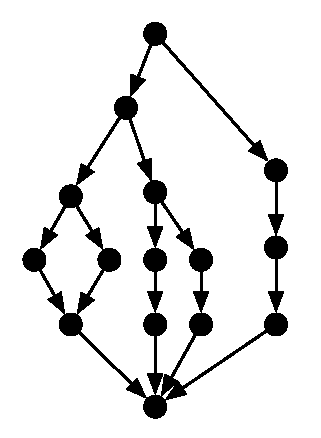
\includegraphics[width=0.4\columnwidth]{pictures/computation-dag}
\fi
\caption{An example computation DAG.}
\label{fig:dag}
\end{figure}



\begin{theorem}[Brent's theorem for computation DAGs]
\label{thm:basic-brent}
Let $G$ be a computation DAG made of $W$ nodes and whose
longest path has length $D$.
%Let $W$ be the number of nodes in $G$ and $D$ be the length of
%the longest path in $G$.
Any greedy scheduler can 
execute this computation DAG in no more than $\frac{W}{P} + D$ 
steps on $P$ processors. 
\end{theorem}
\begin{proof}
At each execution step, each processor places a token in the {\em work bucket}
if it is busy at this step, otherwise it places a token in the {\em idle bucket}.
The work bucket contains exactly $W$ tokens at the end of the execution.
Let $I$ be the number of tokens contained in the idle bucket at the end of the
execution, and let $T$ denote the total number of steps in the execution.
Because a total $T P$ tokens are created, we have $T P = W + I$.
In order to establish the result $T \leq \frac{W}{P} + D$,
it thus suffices to establish the inequality $I \leq P D$.

Consider a given time step.
If all processors are executing then the idle bucket
receives zero tokens. Otherwise, a number of processors are idle.
In this case, the idle bucket receives between one and $P-1$ tokens.
We can bound the number of time steps at which this situation happens,
as follows. 
If one or more processors are idle, it means that those processors cannot
find a ready task to execute. Because the scheduler is assumed to be greedy,
it must be the case that all the ready tasks are currently executing.
Therefore, at such a time step, the maximal length of a path 
in the computation DAG starting from a ready node decreases by one unit. 
Because the maximal length of a path in the computation DAG is initially $D$,
there can be at most $D$ time steps at which not all processors are executing.
It follows that the final number of tokens in the idle bucket
does not exceeed $(P-1) D$. This result entails the inequality $I \leq P D$. \qed
\end{proof}

Observe that the proof does not impose any constraint on the order in
which the ready tasks should be executed by the processors.  So, if one
processor starts working on a sequence of several nodes, then it can
execute all the nodes in the sequence before looking for other ready
tasks.  Therefore, the proof accepts computation DAGs that encode
non-unit tasks as sequences of unit tasks.  We will make use of such
an encoding in the proof of our next theorem, which relates our cost
semantics to the computation DAG model.  

%% We consider here the case of the oracle semantics, for which we encode
%% the costs $\csp$ and $\corc$ by placing additional nodes in the DAG,
%% but a similar construction could be applied for the other evaluation
%% modes.

\begin{theorem}[Brent's theorem for the cost semantics] 
\label{thm:generalize-brent}
\label{thm:generalized-brent}~\\
%Let $e$ be an expression whose total work is $\sws$ and whose total 
%depth is $\sds$. In other words, 
Assume 
$\Jcostof{\sorc}{ e }{ v }{\sw}{\sd}{\sws}{\sds}$
to hold for some $v$, $\sw$ and $\sd$.
Any greedy scheduler can execute the expression $e$
in no more than $\frac{\sws}{P} + \sds$ computations steps on $P$ processors. 
\end{theorem}
\begin{proof}
In order to invoke the version of Brent's theorem that applies 
to computation DAGs, we build the computation DAG associated 
with the execution of the expression $e$, including nodes that
represent the cost of scheduling.
To that end, we describe a recursive algorithm for turning 
an expression $e$ with total work $\sws$ and total depth $\sds$
into a corresponding computation DAG containing $\sws$ nodes and
whose longest path has length $\sds$.
The algorithm follows the structure of the derivation that
$e$ has total work $\sws$ and total depth~$\sds$.
\begin{itemize}
\item If the last rule has zero premises, then $e$ is an atomic expression
and $\sws = \sds = 1$. We build the corresponding DAG as a single node.
\item If the last rule has one premise, then $\sws$ takes the form $\sws{}_1 + 1$
and $\sds$ takes the form $\sds{}_1 + 1$. Let $G_1$ be the DAG corresponding
to the sub-expression described in the premise. We build $G$ by 
extending $G_1$ with one node at the bottom, that is, by
sequentially composing $G_1$ with a DAG made of a single node. 
\item Otherwise the last rule has two premises.
First, consider the case where $e$ is a let-expression. 
$\sws$ takes the form $\sws{}_1 + \sws{}_2 + 1$
and $\sds$ takes the form $\sds{}_1 + \sds{}_2 + 1$.
Let $G_1$ and $G_2$ be the DAGs corresponding to the two sub-expressions.
We build $G$ by sequentially composing $G_1$ with a single node and then 
with $G_2$.
\item Consider now the case of a parallel tuple that is sequentialized.
$\sws$ takes the form $\sws{}_1 + \sws{}_2 + 1 + \corc$
and $\sds$ takes the form $\sds{}_1 + \sds{}_2 + 1 + \corc$.
Let $G_1$ and $G_2$ be the DAGs corresponding to the two branches.
We build $G$ by sequentially composing $1 + \corc$ unit-cost nodes
with the sequential composition of $G_1$ and $G_2$.
\item Finally, consider the case of a parallel tuple that is parallelized.
$\sws$ takes the form $\sws{}_1 + \sws{}_2 + 1 + \csp + \corc$
and $\sds$ takes the form $\kwmax{\sds{}_1}{\sds{}_2} + 1 + \csp + \corc$.
Let $G_1$ and $G_2$ be the DAGs corresponding to the two branches.
We build $G$ by sequentially composing $1 + \csp + \corc$ unit-cost nodes
with the parallel composition of $G_1$ and $G_2$. 
\end{itemize}
It is straightforward to check that, in each case, $\sws$ and $\sds$ 
match the number of nodes and the total depth of the DAG being produced. \qed
\end{proof}


%%%%%%%%%%%%%%%%%%%%%%%%%%%%%%%%%%%%%%%%%%%%%%%%%%%%%%%%%%%%%%%%%%%%%%

\section{Analysis}
\label{sec:analysis}
\label{sec:theorems}

We analyze the impact of task creation overheads on parallel execution
time and show how these costs can be reduced dramatically by using our
oracle semantics.  For our analysis, we first consider an {\em ideal
  oracle} that always makes perfectly accurate predictions (about the
raw work of expressions) without any overhead (\textit{i.e.}, $\corc = 0$).
Such an ideal oracle is unrealistic, because it is practically
impossible to determine perfectly accurately the raw work of
computations.  We therefore consider a realistic oracle that
approximates the raw work of computations by performing constant work.
Our main result is a theorem that shows that the ideal oracle can
reduce the task-creation overheads to any desired constant fraction of
the raw work with some increase in depth, which we show to be small
for a reasonably broad class of computations.

\subsection{Ideal oracle}

We quantify the relationships between raw work, raw depth and
total work, total depth for each mode.

\begin{theorem}[Work and depth]
\label{thm:work-depth-all}
Consider an expression $e$ such that $\Jcostof{\Ga}{ e }{v}{\sw}{\sd}{\sws}{\sds}$.
Assume $\corc = 0$.
The following tight bounds can be obtained for total work and total depth,
on a machine with $P$ processors where the cost of creating parallel tasks is $\csp$.
%
$$\begin{array}{c|c|c} %|l
\X{$\Ga$} & 
\X{Bound on total work} &
\X{Bound on total depth} 

\\\hline
\sseq & 
\sws = \sw &
\sds = \sd = \sw 

\\\hline
\spar & 
\sws \leq (1+\frac{\csp}{2})\,\sw &
\sds \leq (1+\csp)\,\sd 

\\\hline
\sorc & 
\sws \leq (1 + \frac{\csp}{\coff+1})\,\sw &
\sds \leq (1+\kwmax{\csp}{\coff})\,\sd 
\end{array}$$

\end{theorem}

\begin{proof}
The equations concerning the sequential semantics follow by inspection
of the semantics of the source language (\figref{src-sem}).  The
inequalities for the parallel and the oracle modes follow directly by
our more general bounds presented later
(\thmreftwo{orc-cost-depth}{orc-cost-work}).  To prove that the
inequalities for the parallel and the oracles modes are tight, we give
example computation that achieve the bounds.

\begin{itemize}
\item \textbf{Parallel mode.}  Consider an expression consisting only
  of parallel tuples with $n$ leaves, and thus $n-1$ ``internal
  nodes''.  The raw work $\sw$ is equal to $n+(n-1)$ while the total
  work $\sws$ is equal to $n+(n-1)(1+\csp)$.  We therefore have $\sws
  = (1+\frac{n\csp}{2n+1})\sw \le \left(1+\frac{\tau}{2}\right)
  \sw$. As $n$ increases, the bound approaches
  $\left(1+\frac{\tau}{2}\right) \sw$ and thus the bound on the total
  work is tight. To see that the depth bound is also tight, note that
  each parallel tuple adds~$1$ to the raw depth and~$1+\csp$ to the
  total depth.  The total depth therefore can be as much as $1+\csp$
  times greater than the raw depth.

\item \textbf{Oracle mode.}  
Consider an expression with~$n$ nested parallel tuples, where tuples
are always nested in the right branch of their parent tuple.  The
tuples are built on top of expressions that involve~$\coff$ 
units of work.  In the oracle semantics, all the tuples
are executed in parallel.  Thus the raw work~$\sw$ is $n +
(n+1)\coff$, the total work~$\sws$ is $n (1+\csp) +
(n+1)\coff$, and $\sws = \sw \left( 1 + \frac{n\csp}{n(\coff+1)+\coff}
\right) \le \sw \left( 1+\frac{\csp}{\coff+1} \right)$.  As~$n$
increases, the bound approaches $\left(1+\frac{\csp}{\coff + 1}\right) \sw$
and thus the bound on the total work is tight.  

For the depth bound, we  consider two cases.  In the first case,
we have~$\csp \geq \coff$.  Using the same example, the raw depth is~$
\sd = n+1$, the total depth is~$\sds = n(1+\csp) + \coff$, and $\sds =
\left( 1+\frac{n\csp+\coff-1}{n+1} \right) \sd \le \left( 1+\csp
\right) \sd$.  As~$n$ increases,~$\sds$ approaches~$\left( 1+\csp
\right) \sd$ and thus the bound is tight.

For the second case when $\coff\geq\csp$, we change the example
slightly by reducing the amount of raw work in each leaf to just
under $\coff$.  This will cause all the parallel tuples to be
evaluated sequentially; the raw depth is $\sd = n+\coff$ and the
total depth is equal to the total work, \textit{i.e.}, $\sds = n+(n+1)\coff \le
\left( 1+\frac{n\coff}{n+\coff} \right) \sd$.  As $n$ increases, $\sds$
approaches $\left( 1+\coff \right) \sd$ and thus the
bound is tight. \qed
\end{itemize}
\end{proof}

This theorem leads to some important conclusions.  First, the theorem
shows that task creation (scheduling) costs matter a great deal.  In a
parallel evaluation, the total work and total depth can be as much as
$\csp$~times larger than the raw depth and raw work.  This essentially
implies that a parallel program can be significantly slower than its
sequential counterpart.  If $\csp$ is large compared to the number of
processors, then even in the ideal setting, where the number of
parallel processors is small relative to $\csp$, we may observe no
speedups.  In fact, it is not uncommon to hear anecdotal evidence of
this kind of slowdown in modern computer systems.


Second, the theorem shows that evaluation of a program with an ideal
oracle can require as much as $\frac{\coff}{2}$ less work than in the
parallel mode.  This comes at a cost of increasing the depth by a
factor of $\frac{\coff}{\csp}$.  Increasing the depth of a computation can
hurt parallel execution times because many parallel schedulers rely on
the availability of large degree of parallelism to achieve optimal
speedups.  Unless done carefully, increasing the depth can dramatically
reduce parallel slackness.  In the common case, however, where there
is plenty of parallelism, i.e., when $\frac{\sw}{P}$ is far greater
than $\sd$, we can safely increase depth by a factor of
$\frac{\coff}{\csp}$ to reduce the task-creation overheads.
Concretely, if parallel slackness is high and $\coff$ is not too
large, then $\coff\sd$ remains small compared to $\frac{\sw}{P}$, and
$\frac{\csp}{\coff}\frac{\sw}{P}$ becomes much smaller than
$\frac{\csp}{2}\frac{\sw}{P}$,  dramatically reducing task-creation overheads
without harming parallel speedups.

\subsection{Realistic oracles}
\label{sec:realistic-oracles}
\label{sec:estimate}

The analysis that we present above makes two unrealistic assumptions
about oracles: 1) that they can accurately predict the raw work for a
task, and 2) that the oracle can make predictions in zero time.
Realizing a very accurate oracle in practice is difficult, because it
requires determining a priori the execution time of a task.  We
therefore generalize the analysis by considering an approximate or
realistic oracle that can make errors up to a multiplicative factor
$\cerr$ when estimating raw work.  For example, an oracle can
approximate raw work up to a constant factor of~$\cerr=3$,
\textit{i.e.}, a task with raw work $\sw$ would be estimated to
perform raw work between $\frac{\sw}{3}$ and $3\sw$.  Additionally, we
allow the oracle to take some (fixed) constant time, written $\corc$,
to provide its answer.

We show that even with a realistic oracle, we can reduce task creation
overheads.  We start with bounding the depth; the result implies that
the total depth is no larger than $\cerr\coff$ times the raw depth
when $\coff$ is large compared to $\csp$ and $\corc$.  Since with the
ideal oracle this factor was $\coff$, the bound implies that the
imprecision of the oracle can be influenced by changing the
constant multiplicative factor.

%------------------------
\begin{theorem}[Depth with a realistic oracle]
\label{thm:orc-cost-depth}
\label{thm:real-orc-depth}
%Assume an oracle with cost $\corc$ and accurate up to a factor $\cerr$.
$$\Jcostof{\sorc}{ e }{v}{\sw}{\sd}{\sws}{\sds} \Sq\impl \sds \leq (1+\kwmax{\csp}{\cerr\coff}+\corc)\,\sd$$
\end{theorem}
\begin{proof}


Let $\cspp{}$ denote
$1+\kwmax{\csp}{\cerr\coff}+\corc$; we want to  prove that $\sds \leq
\cspp{}\sd$.  The proof is by induction on the derivation 
$\Jcostof{\sorc}{ e }{v}{\sw}{\sd}{\sws}{\sds}$.

$\bullet$  For a rule with zero premises, we have $\sds = \sd = 1$.
Because $\cspp{} \geq 1$, it follows that $\sds \leq \cspp{}\sd$.

$\bullet$  For a rule with one premise, we know by induction hypothesis that
$\sds \leq \cspp{}\sd$.
Using again the fact that $\cspp{} \geq 1$, 
we can deduce the inequality $\sds+1 \leq \cspp{}(\sd+1)$.

$\bullet$ For a rule with two premises, we can similarly establish
the conclusion $\sds{}_1+\sds{}_2+1 \leq \cspp{}(d_1+d_2+1)$ using 
the induction hypotheses 
$\sds{}_1 \leq \cspp{} d_1$ and $\sds{}_2 \leq \cspp{} d_2$.

$\bullet$  Now, consider the case of a parallel tuple.
First, assume that the two branches of this tuple
are predicted to be large.
In this case, the tuple is executed in parallel and the
branches are executed in oracle mode.
We exploit the induction hypotheses
$\sds{}_1 \leq \cspp{} d_1$ and $\sds{}_2 \leq \cspp{} d_2$
to conclude as follows:
%
$$\begin{array}{l@{}l}
\sds & \Sc{=} \kwmax{\sds{}_1}{\sds{}_2} + 1 + \csp + \corc \\
& \Sc\leq \kwmax{ \cspp{}d_1 }{ \cspp{}d_2 } + 1+\kwmax{\csp}{\cerr\coff}+\corc \\
& \Sc\leq \kwmax{ \cspp{}d_1 }{ \cspp{}d_2 } + \cspp{} \\
& \Sc\leq  \cspp{}\, (\kwmax{ d_1 }{ d_2 } + 1) \\
& \Sc{\leq}  \cspp{}\sd
\end{array}$$

$\bullet$  Consider now the case where both branches are predicted
to be small. In this case, the tuple is executed sequentially.
Because the oracle predicts the branches to be smaller
than $\coff$, they must be actually smaller than $\cerr\coff$.
So, we have $w_1 \leq \cerr\coff$ and $w_2 \leq \cerr\coff$.
Moreover, both branches are executed according to the sequential mode,
so we have $\sds{}_1 = w_1$ and $\sds{}_2 = w_2$. 
It follows that $\sds{}_1 \leq \cerr\coff$ and $\sds{}_2 < \cerr\coff$.
Below, we also exploit the fact that 
$\kwmax{ d_1 }{ d_2 } \geq 1$, which comes from the
fact that raw depth is at least one unit.
We conclude as follows:
%Moreover, we have
%
$$\begin{array}{l@{}l}
\sds & \Sc{=} \sds{}_1 + \sds{}_2 + 1 + \corc \\
& \Sc\leq \cerr\coff + \cerr\coff + 1 + \corc \\
& \Sc\leq  (1+\cerr\coff+\corc)*2 \\
& \Sc\leq  (1+\kwmax{\csp}{\cerr\coff}+\corc)\cdot(\kwmax{ d_1 }{ d_2 } + 1) \\
& \Sc\leq  \cspp{}\sd
\end{array}$$

$\bullet$  It remains to consider the case where one branch is predicted
to be smaller than the cutoff while the other branch is 
predicted to be larger than the cutoff.
In this case again, both branches are executed sequentially.
Without loss of generality, assume that the second branch is predicted
to be small. In this case, we have $w_2 \leq \cerr\coff$.
This first branch is thus executed according
to the sequential mode, so we have $\sds{}_2 = d_2 = w_2$. 
It follows that $\sds{}_2 \leq \cerr\coff$.
For the first branch, which is executed according to the oracle mode,
we can exploit the induction hypothesis which is $\sds{}_1 \leq \cspp{}d_1$.
We conclude as follows:
%
$$\begin{array}{l@{}l}
\sds & \Sc{=} \sds{}_1 + \sds{}_2 + 1 + \corc \\
& \Sc\leq \cspp{}d_1 + \cerr\coff + 1 + \corc\\
& \Sc\leq  \cspp{}d_1 + (1+\kwmax{\csp}{\cerr\coff}+\corc) \\
& \Sc\leq  \cspp{} \, (d_1 + 1) \\
& \Sc\leq  \cspp{} \,(\kwmax{ d_1 }{ d_2 } + 1) \\
& \Sc\leq  \cspp{} \sd
\end{array}$$
\qed
\end{proof}
%------------------------

This ends our analysis of the depth. Now, let us look at the work.
The fact that every call to the oracle can induce a cost~$\corc$ can
lead the work to be multiplied by~$\corc$.  For example, consider a
program made of a complete tree built using~$n-1$ sequential tuples,
and leading to $n$ parallel tuples generating $2n$ values as leaves.
The raw work is equal to $(n-1)+n+2n$, and the total work is
$(n-1)+n\corc+2n$.  Thus, $\sws \le \frac{\corc}{4} \sw$ and this is
tight for large values of $n$.  This means that a program executed
according to the oracle semantics can slow down by as much as
$\corc/4$.

The problem with the above example is that the oracle is called
infrequently---only at the leaves of the computation---preventing us
from amortizing the cost of the oracle towards larger pieces of
computations.  Fortunately, most programs do not exhibit this
pathological behavior, because parallel tuples are often performed
close to the root of the computation, allowing us to detect 
smaller pieces of work early. 

One way to prevent the oracle from being
called on smaller pieces of work is to make sure that it is called at
regular intervals.  For proving a strong bound on the
work, we will simply assume that the oracle is not called on small
tasks by restricting our attention to balanced programs. 
To this end, we define balanced programs as programs 
that call the oracle only on expressions that are no smaller 
than some constant $\cbal$ off from the value $\frac{\coff}{\cerr}$,
for some $\cbal \geq 1$. Note that we use $\frac{\coff}{\cerr}$ as
a target and not $\coff$ so as to accomodate possible over-estimations
in the estimations of raw work.
The formal definition follows.

\begin{definition}[Balanced programs]
For $\cbal \ge 1$, a program or expression $e$ is $\cbal$-balanced if
evaluating $e$ in the oracle mode invokes the oracle only for
subexpressions whose raw work is no less than
$\frac{\coff}{\cerr\cbal}$.
\end{definition}
%
Note that if a program is $\cbal$-balanced and 
if $\cbal < \cbal'$, then this program is also $\cbal'$-balanced.
We will later give a sufficient condition for
proving that particular programs are balanced (\sref {sec:balanced}).


%------------------------
\begin{theorem}[Work with a realistic oracle]
\label{thm:orc-cost-work}
\label{thm:real-orc-work}
Assume $\Jcostof{\sorc}{ e }{v}{\sw}{\sd}{\sws}{\sds}$ where $e$ is
a $\cbal$-balanced program.
\[
\sws \Sq\leq \left(1+\frac{\cerr(\csp+\cbal\corc)}{\coff+1} \right)\,{\sw}.
\]

\end{theorem}
\begin{proof}
We establish the following slightly tighter inequality.
$$\sws \Sq\leq \left(1 + \frac{\csp}{\coff/\cerr\Ss{+}1} + \frac{\corc}{\coff/(\cerr\creg)\Ss{+}1} \right)\,\sw.$$
The bound is indeed tighter because $\creg \geq 1$ and $\cerr \geq 1$.
Define $\coffe$ as a shorthand for $\coff/\cerr$
and $\coffr$ as a shorthand for $\coff/(\cerr\creg)$.
Note that, because $\creg \geq 1$, we have $\coffr \leq \coffe$.
Let $\kpos{x}$ be defined as the value $x$ when $x$ is nonnegative and as zero otherwise.
We prove by induction that:
%
$$\begin{lines}
\sws \Sc\leq \sw + \csp \floorfracposn{\sw-\coff}{\coffe + 1} + \corc \floorfracposn{\sw-\coffr}{\coffr +1}
\end{lines}$$
%
This is indeed a strengthened result because we have:
%
$$\begin{array}{ll}
& \begin{lines}
\csp \floorfracposn{\sw-\coffe}{\coffe+1}
\Sc\leq \csp \frac{\sw}{\coffe+1} 
\Sc\leq \frac{\csp}{\coff/\cerr+1}\,\sw
\end{lines} 
\\
\X{and} &
\begin{lines}
\corc \floorfracposn{\sw-\coffr}{\coffr+1}
\Sc\leq \corc \frac{\sw}{\coffr+1} 
\Sc\leq \frac{\corc}{\coff/(\cerr\creg)\Ss{+}1}\,\sw
\end{lines}
\end{array}$$

The proof is conducted by induction on the derivation of the reduction hypothesis.

$\bullet$ For a rule with zero premises, which describe an atomic
operation, we have $\sws = \sw = 1$, so the conclusion is satisfied.

$\bullet$  For a rule with a single premise,
the induction hypothesis is:
$$\begin{array}{@{}l}
\sws \Sc\leq \sw + \csp \floorfracposn{\sw-\coffe}{\coffe+1} + \corc \floorfracposn{\sw-\coffr}{\coffr+1}
\end{array}$$
So, we can easily derive the conclusion:
$$\begin{array}{@{}l}
\sws+1 \Sc\leq (\sw+1) + \csp \floorfracposn{(\sw+1)-\coffe}{\coffe+1} + \corc \floorfracposn{(\sw+1)-\coffr}{\coffr+1}
\end{array}$$

$\bullet$  For a rule with two premises, we exploit the mathematical inequality
$\floorfrac{n}{q}+\floorfrac{m}{q} \leq \floorfrac{n+m}{q}$. We have:
$$\begin{array}{l@{}ll}
\sws & \Sc{=} \sws{}_1 + \sws{}_2 + 1 \\
& \Sc\leq w_1 + \csp \floorfracposn{w_1-\coffe}{\coffe+1} + \corc \floorfracposn{w_1-\coffr}{\coffr+1} \\
& \quad +\; w_2 + \csp \floorfracposn{w_2-\coffe}{\coffe+1} + \corc \floorfracposn{w_2-\coffr}{\coffr+1} + 1 \\
& \Sc\leq \sw + \csp \floorfrac{\kposOf{w_1-\coffe}+\kposOf{w_2-\coffe}}{\coffe+1}  \\ 
& \quad +\; \corc \floorfrac{\kposOf{w_1-\coffr}+\kposOf{w_2-\coffr}}{\coffr+1} \\
\end{array}$$
%
To conclude, we need to establish the following two mathematical inequalities:
$$\begin{lines}
\kposOf{w_1-\coffe}+\kposOf{w_2-\coffe} \Sc\leq \kposOf{(w_1+w_2+1)-\coffe}\\
\kposOf{w_1-\coffr}+\kposOf{w_2-\coffr} \Sc\leq \kposOf{(w_1+w_2+1)-\coffr}
\end{lines}$$
The two equalities can be proved in a similar way. Let us establish the first one.
There are four cases to consider.
First, if both $w_1$ and $w_2$ are less than $\coffe$, then the right-hand side is zero,
so we are done. Second, if both $w_1$ and $w_2$ are greater than $\coffe$,
then all the expressions are nonnegative, and we are left to check the inequality
$w_1-\coffe+w_2-\coffe \leq w_1+w_2+1-\coffe$.
Third, if $w_1$ is greater than $\coffe$ and $w_2$ is smaller than $\coffe$, then
the inequality becomes $\kposOf{w_1-\coffe} \Sc\leq \kposOf{(w_1-\coffe)+(w_2+1)}$,
which is clearly true.
The case $w_1 \geq \coffe$ and $w_2 < \coffe$ is symmetrical.
This concludes the proof.

$\bullet$  Consider now the case of a parallel tuple
where both branches are predicted to involve more than $\coff$ units of work.
This implies $w_1 \geq \coffe$ and $w_2 \geq \coffe$.
In this case, a parallel task is created. 
Note that, because $\coffr \leq \coffe$, we also have 
$w_1 \geq \coffr$ and $w_2 \geq \coffr$. So, all the values
involved in the following computations are nonnegative.
Using the induction hypotheses, we have:
%
$$\begin{array}{l@{}ll}
\sws 
& \Sc{=} \sws{}_1 + \sws{}_2 + 1 + \csp + \corc  \\ 
& \Sc\leq w_1 + \csp \floorfrac{w_1-\coffe}{\coffe+1} + \corc \floorfrac{w_1-\coffr}{\coffr+1} \\
& \quad +\; w_2 + \csp \floorfrac{w_2-\coffe}{\coffe+1} + \corc \floorfrac{w_2-\coffr}{\coffr+1} + 1 + \csp + \corc \\ 
& \Sc\leq (w_1 + w_2 + 1) + \csp (\floorfrac{w_1-\coffe}{\coffe+1} + \floorfrac{w_2-\coffe}{\coffe+1} + 1) \\
& \quad +\;\corc (\floorfrac{w_1-\coffr}{\coffr+1} + \floorfrac{w_2-\coffr}{\coffr+1} + 1)  \\
& \Sc\leq \sw + \csp \floorfrac{(w_1-\coffe)+(w_2-\coffe)+(\coffe+1)}{\coffe+1}  \\
& \quad +\; \corc \floorfrac{(w_1-\coffr)+(w_2-\coffr)+(\coffr+1)}{\coffr+1} \\
& \Sc\leq \sw + \csp \floorfrac{(w_1+w_2+1)-\coffe}{\coffe+1} + \corc \floorfrac{(w_1+w_2+1)-\coffr}{\coffr+1} \\
& \Sc\leq \sw + \csp \floorfrac{\sw-\coffe}{\coffe+1} + \corc \floorfrac{\sw-\coffr}{\coffr+1}  \\
\end{array}$$

$\bullet$  Assume now that the two branches are predicted to be less than the cutoff.
This implies $w_1 \leq \coffe$ and $w_2 \leq \coffe$. Both these tasks
are executed sequentially, so $\sws{}_1 = w_1$ and $\sws{}_2 = w_2$. %by \thmref{seq-work-depth} 
%Moreover, because the term $e$ is executed in the oracle semantics, in means that the 
%branch corresponding to the previous parallel tuple executed contains
%at least $\coffe$ units of work. 
Since the program is $\cbal$-balanced, 
% umut:replaced this with the balanced condition.
%
%By lemma \lemref{regularity-elim}, the regularity assumption ensures
%that
%
we have $w_1 \geq \coffr$
and $w_2 \geq \coffr$. 
Those inequalities ensure that we are able to pay for the cost of calling the oracle,
that is, the cost $\corc$.
Indeed, since we have $w_1 + w_2 + 1 - \coffr \geq \coffr+1$, 
we know that $\floorfrac{w_1 + w_2 + 1-\coffr}{\coffr+1} \geq 1$.
Therefore:
%
$$\begin{array}{l@{}ll}
\sws 
& \Sc{=} \sws{}_1 + \sws{}_2 + 1 + \corc \\ 
& \Sc\leq w_1 + w_2 + 1 + \corc \\
& \Sc\leq (w_1 + w_2 + 1) + \corc \floorfrac{w_1 + w_2 + 1-\coffr}{\coffr+1}  \\
& \Sc\leq \sw + \csp \floorfrac{\kposOf{\sw-\coffe}}{\coffe+1} + \corc \floorfrac{\sw-\coffr}{\coffr+1} \\
\end{array}$$

$\bullet$  It remains to consider the case where one branch
is predicted to be bigger than the cutoff while the other
is predicted to be smaller than the cutoff. For example,
assume $w_1 \geq \coffe$ and $w_2 \leq \coffe$.
The parallel tuple is thus executed as a sequential tuple.
The first task is executed in oracle mode, whereas the
second task is executed in the sequential mode.
For the first task, we can invoke the induction hypothesis
$\sws{}_1 \leq w_1 + \csp \floorfrac{w_1-\coffe}{\coffe+1} + \corc \floorfrac{w_1-\coffr}{\coffr+1} $.
For the second task, which is executed sequentially, we have $\sws{}_2 = w_2$.
Moreover, the regularity hypothesis gives us $w_2 \geq \coffr$.
%This inequality implies $w_2 + 1 \geq \coffe / \creg + 1$, 
Hence, we have $\floorfrac{w_2+1}{\coffr+1} \geq 1$.
We conclude as follows:
%
$$\begin{array}{@{}l@{}ll}
\sws 
& \Sc{=} \sws{}_1 + \sws{}_2 + 1 + \corc \\ 
& \Sc\leq w_1 + \csp \floorfrac{w_1-\coffe}{\coffe+1} 
+ \corc \floorfrac{w_1-\coffr}{\coffr+1} + w_2 + 1 + \corc \\
& \Sc\leq w_1 + \csp \floorfrac{w_1-\coffe}{\coffe+1} 
+ \corc \floorfrac{w_1-\coffr}{\coffr+1} + w_2 + 1 + \corc \floorfrac{w_2+1}{\coffe+1} \\
& \Sc\leq \sw + \csp \floorfrac{w_1+w_2+1-\coffe}{\coffe+1} + \corc \floorfrac{w_1+w_2+1-\coffr}{\coffr+1} \\
& \Sc\leq \sw + \csp \floorfrac{\sw-\coffe}{\coffe+1} + \corc \floorfrac{\sw-\coffr}{\coffr+1} \\
\end{array}$$
\qed
\end{proof}

We are now ready to combine the version of Brent's theorem
adapated to our cost semantics with the bounds that we
have established for the total work and depth 
in $\cbal$-balanced parallel programs executed
under the oracle semantics.

\begin{theorem}[Execution time with a realistic oracle]
\label{thm:orc-cost-bound}
\label{thm:orc-time-bound}~\\
Assume an oracle that costs~$\corc$ and makes an error by a factor not
exceeding~$\cerr$. Assume $\coff > \csp$, which is always the case
in practice.
The execution time of a parallel $\cbal$-balanced
program on a machine with $P$ processors under the oracle semantics
with a greedy scheduler does not exceed the value
%\Jtimeorc{P} = 
\[
\left( 1+\frac{\cerr(\csp+\cbal\corc)}{\coff} \right)\,\frac{\sw}{P} \Sc{+} \left( \coff\cerr + \corc + 1\right)d.
\]
\end{theorem}
\begin{proof}
The bound follows by the version of Brent's theorem
adpated to our cost semantics
(\thmref{generalize-brent}), and by the bounds 
established in
\thmref{orc-cost-work} and \thmref{orc-cost-depth}. 
For simplicity, we have replaced the denominator $\coff+1$
with $\coff$. This change does not loosen the bound significantly
because $\coff$ is usually very large in front of a unit cost.
%The first
%inequality follows by simple arithmetic and the fact that $\coff +
%\cerr > \coff$.  The final inequality follows by simple arithmetic
%using the bounds assumed.
 \qed
\end{proof}

\subsection{Choice of the cutoff}

%------------------------
\begin{figure}
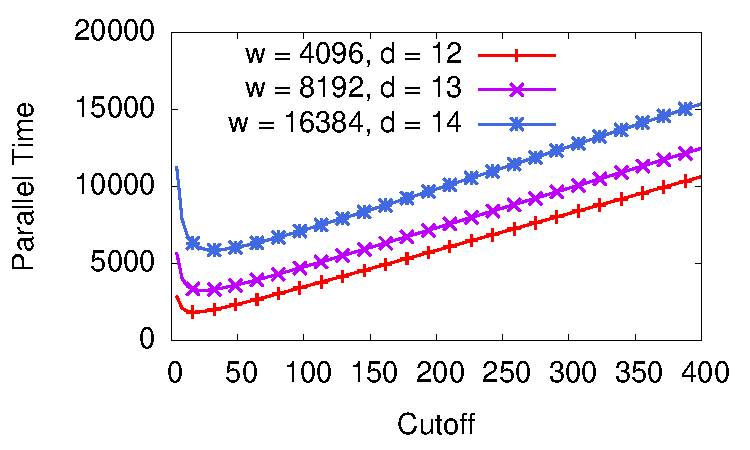
\includegraphics[width=3in]{pictures/plot-run-time-versus-k-multi}

\caption{An illustration of the run-time function $\left(
  1+\frac{\cerr(\csp+\cbal\corc)}{\coff} \right)\,\frac{\sw}{P} \Sc{+}
  (\coff\cerr+\corc+1)\,d$ on $P = 4$ processors with constants $\cerr =1$,
   $\csp = 5$, $\cbal = 1$, and $\corc = 2$, and different work and
  depth values.}

\label{fig:run-time-versus-kappa}
\end{figure}

\thmref{orc-time-bound} shows that the running time of a parallel
program can be controlled by changing the constant $\coff$; the
formula, however, reveals an interesting tradeoff: we can reduce
task-creation overheads but this comes at the cost of increasing the
depth.  To see this connection better, consider the bound
that appears in the statement of \thmref{orc-time-bound}
%$$
%\left( 1+\frac{\cerr(\csp+\creg\corc)}{\coff} \right)\frac{\sw}{P}
%\Sc{+} \left( \coff\cerr + \corc + 1\right)d$$
and notice that as \coff increases the work (first) term decreases
but the depth (second) term increases.  \figref{run-time-versus-kappa}
illustrates a concrete instance of the bound for a hypothetical
computation for fixed constants but different raw work and raw depth.
The exact values of the constant and the raw work and depth are not
relevant to our discussion; constants are fixed at some reasonable
values consistent with our experimental observations.  The work and
depth are consistent with a program whose raw work is linear
in the input size
and whose raw depth is logarithmic in the input size.

As \figref{run-time-versus-kappa} illustrates, the parallel run time
decreases as we increase \coff up to some inflection point and then
starts increasing.  
%ARTHUR: Confirming minimality by checking that the sign of
%the second derivative is positive at the inflection point, 
We compute the optimal value for \coff by solving for the root of the  
derivative. We obtain:
\[
\coff^* = \sqrt{\csp+\creg\corc} \cdot
\sqrt{ \frac{\sw}{P\sd} }.
\]
Thus, with prior knowledge of the raw work and raw depth of a
computation, we can pick \coff to ensure efficiency of parallel
programs.  

Such knowledge, however, is often unavailable.  As we now
show, we can improve efficiency of parallel programs by selecting a
fixed $\coff$ that guarantees that the task creation overheads can be
bounded by any constant fraction of the raw work, without increasing
the depth of the computation significantly. 

%The idea is to make sure that $\coff < \coff^*$, \textit{i.e.}, the cutoff
%remains less than the inflection point.


\begin{theorem}[Run time with fixed $\coff$]
\label{thm:task-creation-overheads}
Consider an oracle with $\corc$ cost and $\cerr$ error.
For any $\cbal\geq 1$ and for any constant $r$ such that $0 < r < 1$,
there exists a constant $\coff$ and a constant $c$
such that the evaluation with 
the oracle semantics of a $\cbal$-balanced program 
reduces task creation overheads to a fraction $r$ of the
raw work, while in the same time increasing the total depth 
by no more than a factor $\frac{c}{r}$.
With a greedy scheduler, the total parallel
run time on $P$ processors of such a program
therefore does not exceed
$(1 + r) \frac{\sw}{P} + \frac{c}{r}\, \sd$.  
%
%When the raw work is a function asymptotically greater than raw depth,
%the increase in depth is not significant: for all but a constant
%number of inputs the total run-time improves over when $\coff = 0$,
%where all parallel tasks are executed in parallel.
\end{theorem}
\begin{proof}
Consider a particular $\cbal$-balanced program 
with raw work $\sw$ and raw depth $\sd$,
%and let $\sw$ denote its raw work and $\sd$ denote its raw depth.
and consider its evaluation under the oracle semantics.  
%
By \thmref{real-orc-work} we know that total work does not exceed
\[
\left(1+\frac{\cerr(\csp+\cbal\corc)}{\coff} \right)\,{\sw}.
\]
To achieve the desired bound on execution time, we take 
 $\coff = \frac{\cerr(\csp + \cbal\corc)}{r}$.
Plugging this value of $\coff$ into the formula
yields~$(1+r)\,{\sw}$ for total work, showing
that task creation overheads are reduced to a fraction $r$ of
the raw work.

Furthermore, by \thmref{real-orc-depth} we know that the total depth 
is bounded by $(\kwmax{\csp}{\cerr\coff}+\corc+1)\,\sd$. Plugging in 
the same value for $\coff$ yields the following bound on total depth:
\[
\sds \Sc\leq \left(\kwmax{\csp}{\frac{\cerr^2(\csp +
    \cbal\corc)}{r}}+\corc + 1\right)\,\sd.
\]
Using $\cerr \ge 1$ and $r < 1$,
we can derive the inequality
\[
\sds \Sc\leq \left(\frac{\cerr^2(\csp + \cbal\corc)}{r}+\frac{\corc+1}{r}\right)\,\sd.
\]
Choosing $c = \cerr^2(\csp + \cbal\corc)+\corc+1$ 
therefore ensures that the total depth does not exceed the desired bound
$\frac{c}{r}\,\sd$.
The run-time bound follows by an application of 
Brent's theorem (\thmref{generalized-brent}). \qed
\end{proof}

This final theorem enables us to reduce task creation overheads to any
desired constant fraction of the raw work by choosing a $\coff$ that
is independent of the specific inputs.  This comes at the cost
of increasing the depth, but only by a constant factor of
$\frac{c}{r}$.  In the common case, when the work is
asymptotically greater than depth, \textit{e.g.}, $\Theta(n)$ versus
$O(\log{n})$, the resulting run-time guarantees that the increase in
depth remain small: specifically, the depth term itself is a fraction
of the work term for all but a constant number of small inputs.  


%% Finally, to show that choosing $r > 0$ improves the run-time for
%% most inputs, we prove that $\coff < \coff^*$ for all but a constant
%% number of inputs when there is an asymptotic gap between work and
%% depth.  The inequality $\coff < \coff^*$ holds if $ \frac{\cerr(\csp +
%%   \cbal\corc)}{r} < \sqrt{\frac{\cerr (\csp+\creg\corc)}{\cerr+1}}
%% \cdot \sqrt{ \frac{\sw}{P\sd}}.  $ Using basic algebra, we deduce that
%% the inequality holds if $r^2 > \cerr(\cerr+1)(\csp + \cbal\corc)
%% \frac{P\sd}{\sw}$.  This can be read simply as $r^2 > c'
%% \frac{P\sd}{\sw}$, where $c'$ is the appropriate constant.  Thus, if
%% there is an asymptotic gap between work and depth, that is
%% $\frac{\sd}{\sw} = o(1)$, then $\frac{\sw}{\sd}$ will increase
%% monotonically with the input size and thus $\coff < \coff^*$ for all
%% input sizes except for some constant number.\qed



\subsection{Balanced programs}
\label{sec:balanced}

Our bounds with the realistic oracle hold only for what we called
$\cbal$-balanced programs, where the oracle is not called on small
tasks.  This assumption can be satisfied by calling the oracle
``regularly.''  It seems likely that this assumption would hold for
many programs without requiring any changes to the program code.  In
this section, we show that recursive, divide-and-conquer programs are
$\cbal$-balanced.

To that end, we introduce the notion of $\cbal$-regularity.
Intuitively, a program is $\cbal$-regular if, between any two calls
to the oracle involved in the execution of this program,
the amount of work does not reduce by more than a factor $\cbal$.
We will then establish that any $\cbal$-regular program is 
a $\cbal$-balanced program.
Before giving the formal definition of $\cbal$-regularity,
we need to formally define what it means for a parallel tuple
to be dominated by another parallel tuple.

\begin{comment}
Fortunately, most programs do not exhibit this pathological behavior.
However, to prove a better bound we need to make further assumptions
about the structure of the program. It turns out that a sufficient
condition for establishing an interesting bound is to ensure
that the oracle is never called on too small tasks.
This property is hard to capture in a hardware-independent way.
However, we can devise a sufficient condition, called {\em regularity},
which is hardware-independent and ensures the desired property. 
Intuitively, a program is $\creg$-regular if the ratio between 
the work involved in a recursive call and the work involved
in the next recursive call does not exceed $\creg$.
Divide-and-conquer algorithm typically satisfy the regularity 
condition. We next formalize the definition of regularity.
\end{comment}

%------------------------
\begin{definition}[Domination of a parallel branch]
A branch $e$ of a parallel tuple is said to be {\em dominated} by the
branch $e_i$ of another parallel tuple $\kwpt{e_1}{e_2}$ if
the expression $e$ is involved in the execution of the branch $e_i$.
\end{definition}
%------------------------

%------------------------
\begin{definition}[Regularity of a parallel program]
A program is said to be $\creg$-regular if,
for any parallel branch involving, say, $\sw$ units of raw work, 
either $\sw$ is very large compared with $\coff/(\cerr\creg)$
or this branch is dominated by another parallel branch
that involves less than $\creg\sw$ units of work.
\end{definition}
%------------------------
%
The condition ``$\sw$ is very large compared with $\coff/(\cerr\creg)$''
is used to handle the outermost parallel tuples, which are not
dominated by any other tuple. 

Note that the regularity of a program is always greater than $2$.
Indeed, if one of the branch of a parallel tuple is more
than half of the size of the entire tuple, then the other 
branch must be smaller than half of that size.
On the one hand, algorithms that divide their work in 
equal parts are $\creg$-regularity with $\creg$ very close to $2$.
On the other hand, ill-balanced programs can have a very
high degree of regularity. Observe that every program is $\infty$-regular.

%------------------------
%\begin{example}[Regularity in a complete binary tree] ~\\
For example, consider a program that traverses a complete binary tree
in linear time. A call on a tree of size $n$ 
has raw work \W{nc}, for some constant $c$.
If the tree is not a leaf, its size $n$ has to be at least $3$.
The next recursive call involves raw work \W{\floorfrac{n-1}{2} c},
The ratio between those two values is equal $n / \floorfrac{n-1}{2}$.
This value is always less than $3$ when $n\geq 3$.
So, the traversal of a complete binary tree is a 3-regular algorithm.
%\end{example}
%------------------------

%------------------------
%\begin{example}[Regularity in mergesort]
%Consider the mergesort algorithm. A recursive call on $2n+1$ values
%has raw work $\Q{c n \log n}$, for some constant $c$.
%A recursive call is performed if $n$ is equal to three or more.
%immediately nested has 
%at least raw work $\Q{c \floorfrac{n-1}{2} \log \floorfrac{n-1}{2}}$,
%So, the ratio between the work of two successive parallel branches is at most:
%$$\frac{c n \log n}{c \floorfrac{n-1}{2} \log \floorfrac{n-1}{2}}$$
%In the worst case, $n=3$, the ratio $2.38$.
%So, merge-sort is $2.38$-regular or less.
%\end{example}
%------------------------

The following lemma explains how the regularity assumption
can be exploited to ensure that the oracle is never
invoked on tasks of size less than $\coff/(\cerr\creg)$.
This suggests that, for the purpose of amortizing well the 
costs of the oracle, a smaller regularity is better.

%------------------------
\begin{lemma}[From regularity to balanced]
\label{lem:regularity-elim}~\\
If a program is $\cbal$-regular then it is $\cbal$-balanced.
\end{lemma}
\begin{proof}
We have to show that, during the execution of a $\creg$-regular 
program according to oracle semantics, the oracle is
never invoked on subexpressions involving less than $\coff/(\cerr\creg)$
raw work.
Consider a particular subexpression $e$ involving $\sw$ units of raw work,
and assume that the oracle is invoked on this subexpression.
Because the oracle is being invoked, $e$ 
must correspond to the branch of a parallel tuple.
By the regularity assumption, either $\sw$ is very
large compared with $\coff/(\cerr\creg)$, in which case
the conclusion holds immediately, or the branch $e$
is dominated by a branch $e_i$ that involves that 
involves $\sw'$ units of work, with $\sw' \leq \creg\sw$.
For the latter case, we need to establish $\sw \geq \coff/(\cerr\creg)$.
To that end, it suffices to prove that $\sw' \geq \coff/\cerr$,
which amounts to showing that the amount of raw
work associated with the dominating branch $e_i$
contains at least $\coff/\cerr$ raw work. 

We conclude the proof by establishing the inequality $\sw' \geq \coff/\cerr$.
Because the oracle is being invoked on the subexpression $e$,
it means that $e$ is being evaluated in the mode $\sorc$. Therefore,
the call to the oracle on the dominating branch $e_i$ must have 
predicted $e_i$ to contain more than $\coff$ raw work.
(Otherwise $e_i$ and its subexpression $e$ would have both
been executed in the sequential mode.)
Given that the oracle makes error by no more than a factor $\cerr$,
if $e_i$ is predicted to contain more than $\coff$ units of raw work, 
then $e_i$ must contain at least $\coff/\cerr$ units of raw work. 
So, $\sw' \geq \coff/\cerr$. \qed
\end{proof}
%------------------------

%%%%%%%%%%%%%%%%%%%%%%%%%%%%%%%%%%%%%%%%%%%%%%%%%%%%%%%%%%%%%%%%%%%%%%
%******************************************************************************
\section{Oracle Scheduling}
%\section{Compilation}
\label{sec:scheduling}
\label{sec:schedule}

\begin{comment}
The original theorem of Brent and our generalization assume a greedy
scheduler that can find available work (parallel tasks to execute)
immediately with no overhead.  This is unrealistic of course but many
schedulers can achieve similar bounds asymptotically for a reasonably
broad class of computations.  For example, a work-stealing scheduler
can execute a fully-strict computations with $\sws$ work and $\sds$
depth on $P$ processors in $O(\sws/P + \sds)$ expected
time~\cite{BlumofeWorkStealing}.  The class of fully-strict
computations (\textit{i.e.}, series-parallel computations) include all
fork-join programs, nested-parallel computations, and specifically
computations with parallel tuples, our focus here.

%\paragraph{Oracle Scheduling.}

Since our oracle semantics makes no assumptions about the specifics of
a scheduler (the semantics simply determines when to create parallel
tasks), the created parallel tasks can be scheduled by using any
suitable scheduler, \textit{e.g.}, a work-stealing scheduler.

%ARTHUR :
In our experiments (\secreftwo{imp}{exp}), we use an implementation of
this estimator combined with a work-stealing scheduler
\end{comment}


As we
describe in this section, we can realize the oracle semantics by using
a {\em $(\corc,\cerr)$-estimator} that requires $\corc$ time to
estimate actual run-time of parallel tasks within a factor of no more
than $\cerr$.  We refer to the combination of an estimator with a
parallel scheduler as an {\em $(\corc,\cerr)$-oracle-scheduler}. 

\begin{figure}
\small
\begin{lstlisting}[language=ocaml]
type cost
type estimator
val create: unit -> estimator

val report: estimator * cost * float -> unit
val predict: estimator * cost -> float
\end{lstlisting}
\caption{The signature of the estimator data structure.}
\label{fig:estimator-sig}
\end{figure}



\paragraph{Run-time estimators.}
To realize the oracle semantics, we require the user to provide a {\em
  cost function} for each function in the program and rely on an {\em
  estimator} for estimating actual work using the user-provided cost
information.  When applied to an argument \ttt{v}, a cost function of
\ttt{f} returns the abstract cost of the application of \ttt{f} to
\ttt{v}. The cost is passed to the estimator, which uses the cost to
compute an estimate of the actual execution time, that is, the raw
work, of the application.  \figref{estimator-sig} shows a signature
for the estimator. To perform accurate estimates, the estimator
utilizes profiling data obtained from actual execution times. The
sampling operation 
%\begin{center}
\ttt{\kwestimatordata(t, c, e)}
%\end{center}
 adds a cost \ttt{c} and an execution time \ttt{e} to the set of
 samples in an estimator \ttt{t}. An estimate of the actual execution
 time is obtained by calling \ttt{predict}.  Given an estimator
 \ttt{t} and cost \ttt{c}, the call
%\begin{center}
\texttt{\kwestimatorapp(t, c)}
%\end{center}
returns a predicted execution time.

%% Note that the exact definition or type of the
%% abstract cost and the nature of the estimator vary as long as they
%% remain consistent: the estimator must be able to interpret the
%% abstract cost in approximating the actual run time.


\paragraph{Compilation.}

To support oracle scheduling with estimators, we need compilation
support to associate an estimator with each function defined in the
program code, to derive a sequential and an oracle version for each
function, and to evaluate tuples sequentially or in parallel depending
on the approximations performed by the estimator.  

For simplicity, we assume that constituents of parallel tuples are
function applications, \textit{i.e.}, they are of the form
$\kwpt{f_1\,v_1}{f_2\,v_2}$.  Note that this assumption does not cause
loss of expressiveness, because a term $e$ can always be replaced by a
trivial application of a ``thunk'', a function that ignores its
argument (typically of type ``unit'') and evaluates $e$ to a dummy
argument. Throughout, we write $\Q{\kwfuncost{f}{x}{e_b}{e_c}}$ to
denote a function $\Q{\kwfun{f}{x}{e_b}}$ for which the cost function
for the body $e_b$ is described by the expression $e_c$.  This
expression $e_c$, which may refer to the argument $x$, should be an
expression whose evaluation always terminates and produces an cost of
type \kwtypeofcost.

To associate an
estimator with each function, in a simple pass over the source code,
we allocate and initialize an estimator for each
syntactic function definition.  For
example, if the source code contains a function of the form
$\Q{\kwfuncost{f}{x}{e_b}{e_c}}$, then our compiler allocates an
estimator specific to that function definition.  Specifically, if the
variable~$r$ refers to the allocated estimator, then the translated
function, written $\Q{\kwfuncostced{f}{x}{e_b}{e_c}{r}}$, 
is annotated with $r$.




%----------
\begin{figure*}

%% \begin{minipage}{\textwidth}
%% \begin{codeListing}
%% fun MeasuredRun (est,c,t) =
%% \\
%% let 
%% \\
%% ~~start = get\_time ()
%% \\
%% ~~v = t ()
%% \\
%% ~~finish = get\_time ()
%% \\
%% ~~() = \kwestimatordata(est,c,finish-start)
%% \\
%% in
%% \\
%% ~~v
%% \\[4mm]
%% %
%% fun Oracle(f,v) = 
%% \\
%% let 
%% \\
%% ~~est = \kwestimatorof{f}
%% \\
%% ~~c = est ((\kwcostfunof{f}) v)
%% \\
%% in
%% \\
%% ~~if c < \coff then
%% \\
%% ~~~~(false, fn () => MeasuredRun (est,c,\kwseqof{f}))
%% \\
%% ~~else
%% \\
%% ~~~~(true, fn () => \kworcof{f})
%% \end{codeListing}

%MeasuredRun\,(r,m,k) \Sc\equiv \\
%\quad\begin{lines}
%\kwletins{t}{\kwappunit{get\_time}} \\
%\kwletins{v}{\kwappunit{k}} \\
%\kwletins{t'}{\kwappunit{get\_time}} \\
%\kwapp{ced\_measured}{(r,m,(t'-t))}; \\
%v
%\end{lines}

%% \caption{Pseudo code for an oracle.}
%% \label{fig:oracle-code}

%% \end{minipage}

%\medskip

\begin{minipage}{\textwidth}
\newcommand{\kwApphere}[2]{\kwapp{#1}{#2}}
\[
\begin{array}{l@{\quad\equiv\quad}l}
\Fcompval{x} & x 
\\[2mm]
\Fcompval{\kwt{v_1}{v_2}} & \kwt{\Fcompval{v_1}}{\Fcompval{v_2}} 
\\[2mm]
\Fcompval{\kwinl{v}} & \kwinl{\Fcompval{v}} 
\\[2mm]
\Fcompval{\kwinr{v}} & \kwinr{\Fcompval{v}} 
\\[2mm]
\Fcompval{\kwfuncostced{f}{x}{e_b}{e_c}{r}} & 
\Lquadruple{r}
{\kwFun{\_}{x}{\Fcomp{\sseq}{e_c}}}
{\kwFun{f}{x}{\Fcomp{\sseq}{e_b}}}
{\kwFun{f}{x}{\Fcomp{\sorc}{e_b}}} 
\\[2mm]
\Fcomp{\Ga}{v} & \Fcompval{v} 
\\[2mm]
\Fcomp{\sseq}{\kwApphere{v_1}{v_2}} & \kwApphere{\kprojof{3}{\Fcompval{v_1}}}{\Fcompval{v_2}} 
\\[2mm]
\Fcomp{\sorc}{\kwApphere{v_1}{v_2}} & \kwApphere{\kprojof{4}{\Fcompval{v_1}}}{\Fcompval{v_2}} 
\\[2mm]
\Fcompga{\kwt{e_1}{e_2}} & \kwt{\Fcompga{e_1}}{\Fcompga{e_2}} 
\\[2mm]
\Fcompga{\kwletin{x}{e_1}{e_2}} & \kwletin{x}{\Fcompga{e_1}}{\Fcompga{e_2}} 
\\[2mm]
\Fcompga{\kwfst{v}} & \kwfst{\Fcompval{v}} 
\\[2mm]
\Fcompga{\kwsnd{v}} & \kwsnd{\Fcompval{v}} 
\\[2mm]
\Fcompga{\kwcase{v}{x}{e_1}{x}{e_2}} & \kwcase{\Fcompval{v}}{x}{\Fcompga{e_1}}{x}{\Fcompga{e_2}} 
\\[2mm]
%\Fcomp{\sseq}{\kwpt{e_1}{e_2}} & \kwt{\Fcomp{\sseq}{e_1}}{\Fcomp{\sseq}{e_2}} \\
\Fcomp{\sseq}{ \kwpt{ \kwApphere{f_1}{v_1} }{ \kwApphere{f_2}{v_2} } } & \kwt{\kwApphere{\kprojof{3}{\Fcompval{f_1}}}{\Fcompval{v_1}}}{\kwApphere{\kprojof{3}{\Fcompval{f_2}}}{\Fcompval{v_2}}} 
\\[2mm]
\Fcomp{\sorc}{ \kwpt{ \kwApphere{f_1}{v_1} }{ \kwApphere{f_2}{v_2} } } & 
\left\{ \begin{array}{@{}l}
\kwletins{(b_1,k_1)}{\ttt{MakeBranch}(\Fcompval{f_1},\Fcompval{v_1})} \\
\kwletins{(b_2,k_2)}{\ttt{MakeBranch}(\Fcompval{f_2},\Fcompval{v_2})} \\
\kwif{(b_1~\kw{\&\&}~b_2)}{ \kwpt{\kwApphere{k_1}{\kwunit}}{\kwApphere{k_2}{\kwunit}} }{ \kwt{\kwApphere{k_1}{\kwunit}}{\kwApphere{k_2}{\kwunit}}  }
\end{array} \right.
\end{array}
\]

\caption{Translation for oracle scheduling.}
\label{fig:compilation}
\end{minipage}

\end{figure*}
%----------

The second pass of our compilation scheme uses the allocated
estimators to approximate the actual raw work of function applications
and relies on an \ttt{MakeBranch} function to determine whether an
application should be run in the oracle or in the sequential mode.
\figref{compilation} defines more precisely the second pass.  We write
$\Fcompval{v}$  for
 the translation of a value $v$, and we write
$\Fcomp{\Ga}{e}$ for the translation of the expression $e$ according to
the semantics $\Ga$, which can be either $\sseq$ or $\sorc$.  When
specifying the translation, we use triples, quadruples, projections,
sequence, if-then-else statements, and unit value; these constructions
can all be easily defined in our core programming language.


Translation of values other than functions does not depend on the mode
and is relatively straightforward.  We translate functions, which are
of the form $\Q{\kwfuncostced{f}{x}{e_b}{e_c}{r}}$, into a quadruple
consisting of the estimator \ttt{r}, a sequential cost function, the
sequential version of the function, and the oracle versions of the
function.  Translation of a function application depends on the
mode. In the sequential mode, the sequential version of the function
is selected (by projecting the third component of the function) and
used in the application.  Similarly, in the oracle mode, the oracle
version of the function is selected and used in the application.  To
translate a tuple, we recursively translate the subexpression, while
preserving the mode.  Similarly, translation of the \ttt{let},
projections, and \ttt{case} constructs are entirely structural.

In the sequential mode, a parallel tuple is turned into a simple tuple.
In the oracle mode, the translation applies the oracle-based scheduling
policy with the aid of the meta-function \ttt{MakeBranch}.  This
meta-function, shown in \figref{metafunctions}, describes
the template of the code generated for preparing the execution of a
parallel tuple.  \ttt{MakeBranch} expects a (translated) function $f$ and
its (translated) argument $v$, and it returns a boolean $b$ indicating
whether the application of $f$ to $v$ is expected to take more or less
time than the cutoff $\coff$, and a thunk $t$ to execute this application.  On
the one hand, if the application is predicted to take more time than
the cutoff (in which case $b$ is true), then the thunk $t$ corresponds
to the application of the 
oracle-semantics version of the function $f$.  On the other
hand, if the application is predicted to take less time than the
cutoff (in which case $b$ is false), then the thunk $t$ corresponds to
the application of the 
sequential-semantics version of the function $f$. Moreover, in the
latter case, the time taken to execute the application sequentially is
measured. This time measure is reported to the estimator by the auxiliary meta-function
\ttt{MeasuredRun} (\figref{metafunctions}), so as to enable
 its approximations.

Observe that the translation introduces many quadruples and
applications of projection functions. However, in practice, the
quadruples typically get inlined so most of the projections can be
computed at compile time.  Observe also that the compilation scheme
involves some code duplication, because every function is translated
once for the sequential mode and once for the oracle mode. In theory,
the code could grow exponentially when the code involves functions
defined inside the body of other functions. In practice, the code the
growth is limited because functions are rarely deeply nested.  If code
duplication was a problem, then we can use flattening to eliminate
deep nesting of local functions, or pass the mode $\Ga$ as an extra
argument to functions.


%----------
\begin{figure}[t]

$$\begin{lines}
\ttt{MakeBranch}\,(f,v) \Sc\equiv \\
\quad\begin{lines}
\kwletins{r}{\kprojof{1}{f}} \\
\kwletins{m}{\kwapp{\kprojof{2}{f}}{v}} \\
\kwletins{b}{\kwestimatorapp(r,m) > \coff} \\
\kwletins{\kw{fun}~k_{\sseq}\,\kwunit}{\kwapp{\kprojof{3}{f}}{v} } \\
\kwletins{\kw{fun}~ k_{\sseq}'\,\kwunit}{\ttt{MeasuredRun}(r,m,k_{\sseq})} \\
\kwletins{\kw{fun}~ k_{\sorc}\,\kwunit}{\kwapp{\kprojof{4}{f}}{v} } \\
\kwletins{k}{\kwif{b}{k_{\sorc}}{k_{\sseq}'}} \\
\kwt{b}{k}
\end{lines}
\\

\ttt{MeasuredRun}\,(r,m,k) \Sc\equiv \\
\quad\begin{lines}
\kwletins{t}{\kwappunit{\ttt{get\_time}}} \\
\kwletins{v}{\kwappunit{k}} \\
\kwletins{t'}{\kwappunit{\ttt{get\_time}}} \\
\kwapp{\kwestimatordata}{(r,m,(t'-t))}; \\
v
\end{lines}
\end{lines}$$

\vspace*{-4mm}

\caption{Auxiliary meta-functions used for compilation.}
\label{fig:metafunctions}
\end{figure}
%----------

\paragraph{Cost as complexity functions.} 

The techniques described in this section require the programmer to
annotate each function defined in the program with a cost function
that, when applied to the argument, returns an abstract cost value.
This abstract cost value is then used by an estimator, which is also
left abstract, to approximate the actual raw work of a task. 
For our bounds to apply, complexity expressions
should require constant time to evaluate.

Predicting the raw work is only needed for sequential tasks,
so the estimator actually needs to return an approximation of the actual run
time of a sequential task.  A crucial property of the abstract cost is
that it should be abstract enough that the programmer can write the
cost functions without necessarily knowing the details of the hardware
that the programs will be executed on.  Yet, abstract costs should
provide sufficient information to estimate the actual run times.   

Asymptotic complexity specifications serve as a natural cost function
by satisfying both of these properties.  Since they eliminate hardware
specific constants, they can be specified easily.  Using complexity
functions, we can approximate the actual run time of sequentially
executed functions by simply determining the constants hidden by the
asymptotic complexity notation.  Such an approximation can be
performed by using the least squares method or similar techniques for
data fitting from known samples.

In our implementation described in \secref{imp}, we implement an
approach based on complexity functions.  We define \kwtypeofcost as an
integer, which represents the application of the complexity function
applied to the input size.  We approximate the actual run time by
calculating a single constant, assuming that the constants in all
terms of the asymptotic complexity are the same.  Although assuming a
single constant can decrease the precision of the approximations, we
believe that it suffices because we only have to compute lower bounds
for our functions; \textit{i.e.}, we only need to determine whether they are
``big enough'' for parallel execution.

%******************************************************************************
%******************************************************************************

\begin{comment}
[TODO: define substitution on language with cost expressions]
[TODO: define the semantics judgment on that language]
[TODO: theorems concern termination but could be extended to divergence]




%-------------------------------------------------------------------
\subsection{Correctness of the translation}

In this section, we outline the proof of correctness for our
translation. For this proof, we introduce a reference semantics whose
judgement takes the form
$$e \redb v$$ where $e$ is a term that evaluates to a value $v$. The
references semantics is similar to the dynamic cost semantics, except
for two cases: For simplicity, the reference semantics does not
measure costs and, as such, does not include oracle derivation rules.
For correctness, the reference semantics has a modified version of the
function-application rule where the cost function is applied to the
same argument as the function and the application is forced to
evaluate to a value. The correctness theorem below, as stated, would
be incorrect otherwise, because without the modification,
nonterminating cost functions could cause translated expressions to
diverge even though their untranslated counterpart expressions
converge.

The substitution lemma shows that our translation commutes with the
substitution of value for a variable inside a source expression.
\begin{lemma}[Substitution]
\label{lem:trans-substitution}
Let $e$ be an expression, $v$ be a value, $x$ be a 
variable and $\alpha$ be either $\sseq$ or $\sorc$.
Then,
$$\Fcomp{\alpha}{e[v/x]} \Sq\equiv
\Fcomp{\alpha}{e}[\Fcompval{v}/x]$$
\end{lemma}
The following two lemmas state the specifications of our metafunctions
$MeasuredRun$ and $MakeBranch$. The proof of each follows trivially from
the definitions.
\begin{lemma}[MeasuredRun]
\label{lem:trans-measured-run}
If $r$, $m$, and $k$ are \src values,
\begin{itemize}
\item $r$ is of type $\Tced$
\item $m$ is of type $\F{int}$
\item $k() \redb v$
\end{itemize}
then $MeasuredRun (r, m, k) \redb v$.
\end{lemma}
\begin{lemma}[Semantics of the function MeasureRun]
\label{lem:trans-run}
Let $r$ be a CED value, $m$ an integer value, $k$ a continuation
and $v$ a value.
If \W{\Jsemof{\kwapp{k}{\kwunit}}{v}}
then \W{\Jsemof{MeasureRun (r,m,k)}{v}}.
\end{lemma}

\begin{lemma}[Semantics of the function MakeBranch]
\label{lem:trans-oracle}
If $r$, $f_c$, $f_s$, $f_p$ are \src expressions, $v_a$ is a \src value,
and
\begin{itemize}
\item $r$ is of type $\Tced$
\item $f_c v_a \redb v_c$
\item $f_p v_a \redb v_r$
\item $f_s v_a \redb v_r$
\end{itemize}
and $(b, k)$ $=$ $Oracle ((r, f_c, f_s, f_p), v_a)$, then $k() \redb
v_r$.
\end{lemma}
Finally, the correctness theorem shows that our translation preserves
the meaning of the given source expression, if the source expression
terminates. It is straightforward to extend the argument to cover
expressions that diverge.
\begin{theorem}[Correctness of the translation]
If $e$ is an expression and $v$ a value such that \W{\Jsemof{e}{v}}, then,
for $\alpha$ equal to either $\sseq$ or $\sorc$,
we have \W{\Jsemof{\Fcomp{\Ga}{e}}{\Fcompval{v}}}.
\end{theorem}

\begin{proof}
By induction on the evaluation derivation $\redb$.
\end{proof}





%----------
\begin{figure}[t]

$$\begin{lines}
\kw{val}\;default\_constant = 1.0
\vspace{4pt}\\
\kw{val}\;nb\_begin = 4
\vspace{4pt}\\
\kw{val}\;nb\_grouped = 20 * nb\_proc 
\vspace{4pt}\\
\kw{val}\;weight = 3
\vspace{4pt}\\

\kw{type}\;\Tced\Sc{=} 
\begin{array}[t]{@{}l@{\;}l@{}l} 
\{ & global & \Sc{:} \kw{float}; \\
& local & \Sc{:} \kw{(bool * int * float)\,array} \,\}  %\Tarray{(\Tbool\Tprod\Tint\Tprod\Tfloat)}
\end{array}
\vspace{4pt}\\

\kw{val}\;ced\_initialize\,() =\\
\quad
\begin{array}[t]{@{}l@{\;}l@{}l} 
\{ & global & \Sc{=} default\_constant; \\
& local & \Sc{=} \kw{make\_array}\,(nb\_proc,\,(\kw{true},\, 0,\, 0.0)) \,\} 
\end{array}
\vspace{4pt}\\

\kw{val}\;ced\_estimate\,(r,m) = m * r.global
\vspace{4pt}\\

\kw{val}\;ced\_report\,(r,c) =\\
\quad \begin{lines}
r.shared \leftarrow (r.shared * weight + c) \Ss/ (weight + 1)
\end{lines}
\vspace{4pt}\\

\kw{val}\;ced\_measured\,(r,m,t) =\\
\quad \begin{lines}
\kwletins{p}{\kwappunit{get\_proc\_id}} \\
\kwletins{(g,n,s)}{ r.\kwarrget{local}{p}} \\
\kwletins{g'}{g~\kw{\&\&}~(n<nb\_begin)} \\
\kwletins{n'}{n+1} \\
\kwletins{s'}{s+(t / m)} \\
\kwletins{c}{s' \Sc/ n'} \\
\kw{if}~g'~\kw{then}~ced\_report\,(r,c); \\
\kw{if}~n' = nb\_grouped~\kw{then}~\kw{begin}\\
\qquad ced\_report\,(r,c); \\
\qquad r.\kwarrget{local}{p} \leftarrow (\kw{false},\, 0,\, 0.0); \\
\kw{end}~\kw{else} \\
\qquad r.\kwarrget{local}{p} \leftarrow (g',\,n',\,s'); \\
\end{lines}
\end{lines}$$

\caption{Auxiliary meta-functions used for compilation}
\label{fig:ced-implementation}
\end{figure}
%----------

\end{comment}


%-------------------------------------------------------------------
\section{Implementation}
\label{sec:imp}

In this section, we describe the implementation of our scheduling
technique in an actual language and system. In our approach, source
programs are written in our own dialect of the 
Caml language~\cite{objective-caml}, which is 
a strict functional language. 
Our Caml dialect corresponds to the core Caml language
extended with syntax for parallel pairs and complexity annotations. 
\figref{exampleprog} shows a program implemented in our Caml dialect.
This recursive program traverse a binary
tree to compute the sum of the values stored in the leaves.
 
%------------------------------
\begin{figure}[t]
\begin{verbatim}
type tree = 
  | Leaf of int 
  | Node of int * tree * tree

let size = function
  | Leaf _ -> 1
  | Size (s,_,_) -> s

let rec sum t = Oracle.complexity (size t);
  match t with
  | Leaf n -> n  
  | Node (size,t1,t2) ->
     let (n1,n2) = (| sum t1, sum t2 |) in
     n1 + n2
\end{verbatim}
\caption{An example parallel program.}
\label{fig:exampleprog}
\end{figure}
%------------------------------

We use the Caml type checker to obtain a typed syntax tree, on which
we perform the oracle-scheduling translation defined in Figure
\ref{fig:compilation}. We then produce code in the syntax
of Parallel~ML (PML)~\cite{FluetRaReSh11}, a parallel 
language close to Standard~ML. The translation from Caml
to PML is straightforward because the two languages are 
relatively similar.
We compile our source programs to x86-64 binaries using Manticore,
which is the optimizing PML compiler. The Manticore run-time system
provides a parallel, generational garbage collector that is crucial
for scaling to more than four processors, because functional programs,
such as the ones we consider, often involve heavy garbage-collection
loads. Further details on Manticore can be found
elsewhere~\cite{Fluet:2008:SFG:1411204.1411239}.
In the rest of this section, we explain how we compute
the constant factors, and we also give a high-level description 
of the particular work-stealing scheduler on top of which 
we are building the implementation of our oracle scheduler.

%-------------------------------------------------------------------
\paragraph{Run-time estimation of constants.}

The goal of the oracle is to make relatively accurate execution 
time predictions at little cost. Our approach to implementing
the oracle consists of evaluating a user-provided asymptotic
complexity function, and then multiplying the result by an
appropriate constant factor. Every function has its own constant
factor, and the value for this constant factor is stored in the
estimator data structure.
In this section, we discuss the pratical implementation of the 
evaluation of constant factors.

In order for the measurement of the constant to be lightweight, we
simply compute average values of the constant.  The constant might
evolve over time, for example if the current program is sharing the
machine with another program, a series of memory reads by the other
program may slow down the current program.  For this reason, we do not
just compute the average across the entire history, but instead
maintain a moving average, that is, an average of the values gathered
across a certain number of runs.

Maintaining averages is not entirely straightforward.
One the one hand, storing data in a memory cell 
that is shared by all processors is not satisfying because it would involve 
some synchronization problems. On the other hand, using a
different memory cell for every processor is not satisfying either,
because it leads to slower updates of the constants when they change.
In particular, in the beginning of the execution of a program
it is important that all processors quickly share a relatively good
estimate of the constant factors.
For these reasons, we have opted for an approach that
uses not only a shared memory cell but also one data structure
local to every processor. 

The shared memory cell associated with each estimator contains the
estimated value for the constant that is read by all the processors
when they need to predict execution times. The local data structures
are used to accumulate statistics on the value of the constant. Those
statistics are reported on a regular basis to the shared memory cell,
by computing a weighted mean between the value previously stored in
the shared memory cell and the value obtained out of the local data
structure. We treat initializations somewhat specially: for the first
few measures, a processor always begins by reporting its current
average to the shared memory cell. This ensures a fast propagation of
the information gathered from the first runs, so as to quickly improve
the accuracy of the predictions.

When implementing the oracle, we faced three technical difficulties.
First, we had to pay attention to the fact that the memory cells
allocated for the different processors are not allocated next to each
other. Otherwise, those cells would fall in the same cache line, in
which case writing in one of these cells would make the other cells be
removed from caches, making subsequent reads more costly.  Second, we
observed that the time measures typically yield a few outliers.  Those
are typically due to the activity of the garbage collector or of
another program being scheduled by the operating system on the same
processor.  Fortunately, we have found detecting these outliers to be
relatively easy because the measured times are at least one or two
orders of magnitude greater than the cutoff value.  Third, the default
system function that reports the time is only accurate by one
microsecond. This is good enough when the cutoff is greater than 10
microseconds.  However, if one were to aim for a smaller cutoff, which
could be useful for programs exhibiting only a limited amount of
parallelism, then more accurate techniques would be required, for
example using the specific processor instructions for counting the
number of processor cycles.

\paragraph{Work stealing.}

We implement our oracle scheme on top of the work stealing
scheduler~\cite{BlumofeWorkStealing}. In this section we outline the
particular implementation of work stealing that we selected from the
Manticore system. Our purpose is to understand what exactly
contributes to the scheduling cost $\tau$ in our system.
% and show that it is reasonable to treat $\tau$ as a constant. 
% -> could it be something  else than "a constant"?

In Manticore's work-stealing scheduler, all system processors are
assigned to collaborate on the computation. Each processor owns a
deque (doubly-ended queue) of tasks represented as thunks. Processors
treat their own deques like call stacks.  When a processor starts to
evaluate a parallel-pair expression, it creates a task for the second
subexpression of the pair and pushes the task onto the bottom of the
deque. Processors that have no work left try to 
{\em steal} tasks from others. More precisely, they repeatedly select 
a random processor and try to pop a task from this processor's deque. 

Manticore's implementation of work stealing~\cite{rainey:phd} adopts a
code-specialization scheme, called clone translation, taken from Cilk-5's
implementation~\cite{FrigoLeRa98}. (In the Cilk-5
implementation, it is called clone compilation.) With clone
translation, each parallel-pair expression is compiled into two
versions: the fast clone and the slow clone. 
The purpose of a fast clone is to optimize the code that corresponds
to evaluating on the local processor,
whereas the slow clone is used when the second branch 
of a parallel-pair is migrated to another processor.
% -> i think the next sentence is already said by the above
%The slow clone executes when
%the second subexpression of the parallel-pair expression is stolen,
%and the fast clone executes otherwise. 
A common aspect of between clone translation and our oracle
translation (Figure \ref{fig:compilation}) is that both generate
specialized code for the sequential case. But the clone translation
differs in that there is no point at which parallelism is cut off
entirely, as the fast clone may spawns subtasks.

The scheduling cost involved in the fast clone is a (small) constant,
because it involves just a few local operations, but the scheduling
cost of the slow clone is variable, because it involves
inter-processor communication. 
It is well established, both through analysis and
experimentation, that (with high probability)
no more than $O(P\sds)$ steals occur during 
the evaluation~\cite{BlumofeWorkStealing}.
So, for programs that exhibit parallel slackness ($\sws \gg P \sds $),
we do not need to take into account the cost of slow clones
because there are relatively few of them.
We focus only on the cost of creating fast clones,
which correspond to the cost $\tau$.
A fast clone needs to packages a task, push it onto the deque
and later pop it from the deque. So, a fast clone is not quite
as fast as the corresponding sequential code.
The exact slowdown depend on the implementation, but in our
case we have observed that a fast clone is 3 to 5 
times slower than a simple function call.


%% Intuitively, the work stealing provides such low scheduling costs
%% because of two properties. First, each processor is assigned its own
%% subgraph of the computation. Processors focus exclusively on executing
%% their own subgraphs before looking for other work.  Idle processors
%% who run out of local work bear the majority of the scheduling
%% costs. Second, when a subgraph is divided between processors, it is
%% usually divided into two large subgraphs of roughly-equal size. This
%% division of subgraphs is called stealing because the division is
%% initiated by an idle processor. The second property helps ensure that
%% few steals happen in total. Processors thus spend most of their time
%% working independently on local subcomputations.

\section{Empirical Evaluation}
\label{sec:exp}
\label{sec:empirical-evaluation}

In this section, we evaluate the effectiveness of our implementation
through several experiments. We consider results from a range of
benchmarks run on two machines with different architectures. The
results show that, in each case, our oracle implementation improves on
the plain work-stealing implementation. Furthermore, the results show
that the oracle implementation scales well with up to sixteen processors.

%-------------------------------------------------------------------
\paragraph{Machines.}

Our AMD machine has four quad-core AMD Opteron 8380 processors running
at 2.5GHz.  Each core has 64Kb each of L1 instruction and data cache,
and a 512Kb L2 cache. Each processor has a 6Mb L3 cache that is shared
with the four cores of the processor.  The system has 32Gb of RAM and
runs Debian Linux (kernel version 2.6.31.6-amd64).

Our Intel machine has four eight-core Intel Xeon X7550 processors
running at 2.0GHz. Each core has 32Kb each of L1 instruction and
data cache and 256 Kb of L2 cache. Each processor has an 18Mb L3 cache
that is shared by all eight cores. The system has 1Tb of RAM and runs
Debian Linux (kernel version 2.6.32.22.1.amd64-smp).
For uniformity, we consider results from just sixteen out of the
thirty-two cores of the Intel machine. 

%-------------------------------------------------------------------
\paragraph{Measuring scheduling costs.}

We report estimates of the task-creation overheads for each of our test
machines. To estimate, we use a synthetic benchmark expression $e$
whose evaluation sums integers between zero and 30 million using a
parallel divide-and-conquer computation. We chose this particular
expression because most of its evaluation time is spent evaluating
parallel pairs. 

First, we measure $w_s$: the time required for executing a
sequentialized version of the program (a copy of the program where
parallel tuples are systematically replaced with sequential tuples).
This measure serves as the baseline.  Second, we measure $w_w$: the
time required for executing the program using work stealing, on a
single processor.  This measure is used to evaluated $\csp$.  Third,
we measure $w_o$: the time required for executing a version of the
program with parallel tuples replaced with ordinary tuples but where
we still call the oracle. %to predict the time and measure the time.
This measure is used to evaluate $\corc$.

We then define the work-stealing overhead $c_w = \frac{w_w}{w_s}$.
We estimate the cost $\csp$ of creating a parallel task in work stealing
by computing $\frac{w_w - w_s}{n}$, where
$n$ is the number of parallel pairs evaluated in the program.
%We obtained the value for $n$ by analysing the program.
We also estimate the cost $\phi$ of invoking the oracle  by computing $\frac{w_o - w_s}{m}$,
where $m$ is the number of times the oracle is invoked.
%We used a runtime counter in the oracle to measure $m$.
Our measures are as follows.
%
\begin{center}
\begin{tabular}{l | c c c c}
Machine & $c_w$  &  $\csp$ ($\mu$s) & $\phi$ ($\mu$s) \\
\hline
AMD   & 4.86   & 0.09  & 0.18 \\
Intel & 3.90  &  0.18  & 0.94 \\
\end{tabular}
\end{center}

\begin{comment}
\begin{center}
\begin{tabular}{l | c c c c}
Machine & $c_w$  & $c_o$ &  $\csp$ ($\mu$s) & $\phi$ ($\mu$s) \\
\hline
AMD   & 4.86  & 8.25 & 0.09  & 0.18 \\
Intel & 3.90 & 7.27 &  0.18  & 0.94 \\
\end{tabular}
\end{center}
\end{comment}

   \begin{comment}
   \begin{center}
   \begin{tabular}{l | c c }
   Machine & $c_w$ & $\csp$ ($\mu$s) \\
   \hline
   AMD   & 4.86 & 0.09 \\
   Intel & 3.90 & 0.18 \\
   \end{tabular}
   \end{center}
   \end{comment}
The first column indicates that work stealing alone can induce
a slowdown by a factor of 4 or 5, for programs that create a
huge number of parallel tuples. 
Column two indicates that the cost of creating parallel task $\csp$ 
is significant, taking roughly between 200 and 350 processor cycles. 
The last column suggests that the oracle cost $\corc$
is of the same order of magnitude ($\corc$ is 2 to 5 times larger than $\csp$).
%It also suggests that slowdown due to scheduling cost can more than 
%double if we execute an oracle but do not exploit its results appropriately.

To determine a value for $\coff$, we use the formula
$\frac{\cerr(\csp+\creg\corc)}{r}$ from \sref{sec:estimate}.  Recall
that $r$ is the targette overhead for scheduling costs.  We aim for $r =
10\%$.  Our oracle appears to be always accurate within a factor 2, so
we set $\cerr = 2$.  Our benchmark programs are fairly regular, so we
take $\creg = 3$.  We then use the values for $\csp$ and $\corc$
specific to the machine and evaluate the formula
$\frac{\cerr(\csp+\creg\corc)}{r}$.  We obtain $13\mu s$ for the AMD
machine and $60\mu s$ for the Intel machine.  However, we were not able to
use a cutoff as small as $13\mu s$ because the time function that we
are using is only accurate up to $1\mu s$.  For this reason, we
doubled the value to $26\mu s$.  (One possibility to achieve greater
accuracy would be to use architecture-specific registers that are able
to report on the number of processor cycles involved in the execution
of a task.)

In our experiments, we used $\coff = 26\mu s$ on the AMD machine and $\coff = 61\mu s$ on the Intel machine.

% insert \kappa here

\begin{figure*}
\begin{center}
  \begin{tabular}{p{3.25in}@{\hfil}p{3.25in}}
    \begin{center}
      AMD
      \medfig{pictures/work-stealing-vs-oracle--for--machine=hexi--proc=16.pdf}
    \end{center}%
    &
    \begin{center}
      Intel
      \medfig{pictures/work-stealing-vs-oracle--for--machine=srv-53-07--proc=16.pdf}
    \end{center}%
  \end{tabular}
\end{center}
\vspace*{-6mm}
\caption{Comparison of the speedup on sixteen processors. Higher bars
  are better.}
\label{fig:comparison-oracle-work-stealing}
\end{figure*}

\begin{figure*}
\begin{center}
  \begin{tabular}{p{3.25in}@{\hfil}p{3.25in}}
    \begin{center}
      AMD
      \medfig{pictures/sequential-vs-oracle-vs-work-stealing--for--machine=hexi--proc=1.pdf}
    \end{center}%
    &
    \begin{center}
      Intel
      \medfig{pictures/sequential-vs-oracle-vs-work-stealing--for--machine=srv-53-07--proc=1.pdf}
    \end{center}%
  \end{tabular}
\end{center}
\vspace*{-6mm}
\caption{Comparison of execution times (normalized) on a single
  processor. Lower bars are better.}
\label{fig:comparison-sequential-oracle-work-stealing}
\end{figure*}


%-------------------------------------------------------------------
\paragraph{Benchmarks.}

We used five benchmarks in our empirical evaluation. Each benchmark
program was originally written by other researchers and ported to our
dialect of Caml. 

The Quicksort benchmark sorts a sequence of 2 million integers. Our
program is adapted from a functional, tree-based
algorithm~\cite{BlellochGr95}. The algorithm runs with $O(n
\log n)$ raw work and $O(\log^2 n)$ raw depth, where $n$ is the length
of the sequence. Sequences of integers are represented as binary trees
in which sequence elements are stored at leaf nodes and each internal
node caches the number of leaves contained in its subtree.

The Quickhull benchmark calculates the convex hull of a sequence of
3 million points contained in 2-d space. The algorithm runs with $O(n
\log n)$ raw work and $O(\log^2 n)$ raw depth, where $n$ is the length
of the sequence. The representation of points is similar to that of
Quicksort, except that leaves store 2-d points instead of integers.

The Barnes-Hut benchmark is an $n$-body simulation that calculates the
gravitational forces between $n$ particles as they move through 2-d
space~\cite{barnes-hut}. The Barnes-Hut computation consists of two
phases. In the first, the simulation volume is divided into square
cells via a quadtree, so that only particles from nearby cells need to
be handled individually and particles from distant cells can be
grouped together and treated as large particles. The second phase
calculates gravitational forces using the quadtree to accelerate the
computation. The algorithm runs with $O(n \log n)$ raw work and
$O(\log n)$ raw depth. Our benchmark runs 10 iterations over 100,000
particles generated from a random Plummer
distribution~\cite{plummer-distribution}. The program is adapted from
a Data-Parallel Haskell
program~\cite{PeytonJonesHarnessingMulticores}. The representation we
use for sequences of particles is similar to that of Quicksort.

The SMVM benchmark multiplies an $m \times n$ matrix with an $n \times
1$ dense vector. Our sparse matrix is stored in the compressed
sparse-row format. The program contains parallelism both between dot
products and within individual dot products. We use a sparse matrix
of dimension $m =$ 500,000 and $n =$ 448,000, containing 50,400,000
nonzero values.

The DMM benchmark multiplies two dense, square $n \times n$ matrices
using the recursive divide-and-conquer algorithm of Frens and
Wise~\cite{FrensWiseAutoblockingDMM}. We have recursion go down to
scalar elements. The algorithm runs with $O(n^3)$ raw work and $O(\log
n)$ raw depth. We selected $n=$ 512.

%-------------------------------------------------------------------
\paragraph{Implementing complexity functions.}

Our aim is to make complexity functions fast, ideally constant time,
so that we can keep oracle costs low. But observe that, in order to
complete in constant time, the complexity function needs access to the
input size in constant time. For four of our benchmark programs, no
modifications to the algorithm is necessary, because the relevant data
structures are already decorated with sufficient size information.
The only one for which we make special provisions is SMVM. The issue
concerns a subproblem of SMVM called segmented
sums~\cite{cray-mvmult}. In segmented sums, our input is an array of
arrays of scalars, \textit{e.g.},
\begin{displaymath}
[[8, 3, 9], [2], [3, 1] [5]]
\end{displaymath}
whose underlying representation is in segmented format. The segmented
format consists of a pair of arrays, where the first array contains
all the elements of the subarrays and second contains the lengths of
the subarrays.
\begin{displaymath}
([8, 3, 9, 2, 3, 1, 5], [3, 1, 2, 1])
\end{displaymath}
The second array is called the segment descriptor. The objective is to
compute the sum of each subarray,
\begin{displaymath}
[20, 2, 4, 5],
\end{displaymath}
There are two sources of parallelism in segmented sums: (1) within
the summation of each subarray and (2) between different subarray
sums. We use divide-and-conquer algorithms to solve each case. In the
first case, our algorithm is just an array summation, and
thus the complexity function is straightforward to
compute in constant time from the segment descriptor. The second
case is where we make the special provisions. For this case, we use a
parallel array-map algorithm to compute all the subarray sums in
parallel. The issue is that the complexity of performing a group of subarray
sums is proportional to the sum of the sizes of those subarrays. So,
to obtain this size information in constant time, we modify our
segmented-array representation slightly so that we store a cached tree
of subarray sizes rather than just a flat array of subarray sizes.
\begin{center}
$([8, 3, 9, 2, 3, 1, 4, 5],$ \Tree [.7 [ 3 1 ].4 [2 1 ].3 ] $)$
\end{center}
To summarize, in order to write a constant-time complexity function,
we changed the existing SMVM program to use a tree data structure,
where originally there was an array data structure. Building the tree
can be done in parallel, and the cost of building can be amortized
away by reusing the sparse matrix multiple times, as is typically done
in iterative solvers.


\begin{figure}
\vspace*{-0.5in}
\centering
%      \smallfig{pictures/speedup--vs--processors--for--barnes-hut--size=100000--param=0--optim=0--machine=hexi.pdf}

      \smallfig{pictures/speedup--vs--processors--for--barnes-hut--size=100000--param=0--optim=0--machine=srv-53-07.pdf}

%      \smallfig{pictures/speedup--vs--processors--for--quicksort--size=2000000--param=0--optim=0--machine=hexi.pdf}

      \smallfig{pictures/speedup--vs--processors--for--quicksort--size=2000000--param=0--optim=0--machine=srv-53-07.pdf}

%      \smallfig{pictures/speedup--vs--processors--for--quickhull--size=2000000--param=0--optim=0--machine=hexi.pdf}

      \smallfig{pictures/speedup--vs--processors--for--quickhull--size=3000000--param=0--optim=0--machine=srv-53-07.pdf}

%      \smallfig{pictures/speedup--vs--processors--for--dmm--size=9--param=0--optim=0--machine=hexi.pdf}

      \smallfig{pictures/speedup--vs--processors--for--dmm--size=9--param=0--optim=0--machine=srv-53-07.pdf}

%      \smallfig{pictures/speedup--vs--processors--for--smvm--size=50000000--param=0--optim=0--machine=hexi.pdf}

      \smallfig{pictures/speedup--vs--processors--for--smvm--size=50000000--param=0--optim=0--machine=srv-53-07.pdf}

\caption{Comparison between work stealing and oracle.}
\label{fig:comparison-ws-oracle}
\end{figure}%


%% \begin{figure*}
%% \begin{center}
%% \bigfig{pictures/tree-inaccurate-costs.pdf}
%% \bigfig{pictures/dmm-inaccurate-costs.pdf}
%% \end{center}
%% \caption{The effects of having inaccurate cost functions}
%% \label{fig:inaccurate-costs}
%% \end{figure*}

%-------------------------------------------------------------------
\paragraph{Performance.}

For every benchmark, we measure several values.
$T_\sseq$ denotes
the time to execute the sequential version of the program.
We obtain the sequential version of the program by replacing each 
parallel tuple with an ordinary tuple and erasing complexity functions,
so that the sequential version includes none of the task-creation overheads.
$T_\spar^P$ denotes the execution time with work stealing on $P$ processors.
$T_\sorc^P$ denotes the execution time of our 
oracle-based work stealing on $P$ processors.

The most important results of our experiments come from comparing
plain work stealing and our oracle-based work stealing side by
side. Figure \ref{fig:comparison-oracle-work-stealing} shows the
speedup on sixteen processors for each of our benchmarks,
that is, the values $T_\spar^{16}/T_\sseq$ and $T_\sorc^{16}/T_\sseq$.
The speedups show that, on sixteen cores, our oracle implementation is
always between 4\% and 76\% faster than work stealing. 

The fact that some benchmarks benefit more from our oracle implementation 
than others is explained by Figure
\ref{fig:comparison-sequential-oracle-work-stealing}. This plot shows
execution time for one processor, normalized with respect to the  
sequential execution times. In other words, the values plotted
are 1, $T_\sorc^{1}/T_\sseq$ and $T_\spar^{1}/T_\sseq$.
The values $T_\sorc^{1}/T_\sseq$ range from 1.03 to 1.13 (with an average
of $1.07$), indicating that the task-creation overheads in the oracle 
implementation do not exceed 13\% of the raw work in any benchmark.
The cases where we observe large improvements in speedup are the same
cases where there is a large difference bewteen sequential execution
time and plain work-stealing execution time. When the difference is
large, there is much room for our implementation to improve on work
stealing, whereas when the difference is small
we can only improve the execution time by a limited factor.
%-> arthur: I don't see the point of this sentence; it's just weakening our results it seems
%The plots show that, where there is much room for
%improvement, our oracle implementation does well, and where there is
%little room, our oracle implementation never does worse.

Figure \ref{fig:comparison-ws-oracle} shows speedup curves for each of
our experiments, that is, values of $T_\spar^{P}/T_\sseq$ and 
$T_\sorc^{P}/T_\sseq$ against the number of processors~$P$ on our
Intel machine; the measurements on the AMD machine show similar trends
but quantitatively better results for the oracle versions.   

%Observe that on the Intel machine there is super-linear scaling, 
%but not on the AMD machine. We attribute this behavior to cache effects.
% ARTHUR: I do not understand what this means:
%We attribute this behavior to
%opportunities for prefetching missed by the sequential program.
The curves show that our oracle implementation generally scales
well up to sixteen processors.

There is one exception, which is the quickhull benchmark on the AMD
machine. For this benchmark, the curve tails off after reaching twelve
processors. We need to conduct further experiments to understand the
cause, which is probably due to a lack of parallelism in the program.
Notice, however, that our scheduler does not fall below work stealing.

%Notice, however, that the curve of plain work stealing
%does not tail off, but approaches the oracle implementation curve from
%below. The work-stealing scheduler is able to utilize the extra
%parallelism to mask scheduling costs. This behavior shows that in this
%case where parallelism is limited, our scheduler does not fall below
%work stealing.





%% \begin{figure*}
%% \vspace*{-0.5in}
%% \begin{center}
%%   \begin{tabular}{p{3.25in}@{\hfil}p{3.25in}}
%%     \begin{center}
%%       \smallfig{pictures/speedup--vs--processors--for--barnes-hut--size=100000--param=0--optim=0--machine=hexi.pdf}
%%     \end{center}%
%%     &
%%     \begin{center}
%%       \smallfig{pictures/speedup--vs--processors--for--barnes-hut--size=100000--param=0--optim=0--machine=srv-53-07.pdf}
%%     \end{center}%
%%     \\[-3em]
%%     \begin{center}
%%       \smallfig{pictures/speedup--vs--processors--for--quicksort--size=2000000--param=0--optim=0--machine=hexi.pdf}
%%     \end{center}%
%%     &
%%     \begin{center}
%%       \smallfig{pictures/speedup--vs--processors--for--quicksort--size=2000000--param=0--optim=0--machine=srv-53-07.pdf}
%%     \end{center}%
%%     \\[-3em]
%%     \begin{center}
%%       \smallfig{pictures/speedup--vs--processors--for--quickhull--size=2000000--param=0--optim=0--machine=hexi.pdf}
%%     \end{center}%
%%     &
%%     \begin{center}
%%       \smallfig{pictures/speedup--vs--processors--for--quickhull--size=3000000--param=0--optim=0--machine=srv-53-07.pdf}
%%     \end{center}%
%%     \\[-3em]
%%     \begin{center}
%%       \smallfig{pictures/speedup--vs--processors--for--dmm--size=9--param=0--optim=0--machine=hexi.pdf}
%%     \end{center}%
%%     &
%%     \begin{center}
%%       \smallfig{pictures/speedup--vs--processors--for--dmm--size=9--param=0--optim=0--machine=srv-53-07.pdf}
%%     \end{center}%
%%     \\[-3em]
%%     \begin{center}
%%       \smallfig{pictures/speedup--vs--processors--for--smvm--size=50000000--param=0--optim=0--machine=hexi.pdf}
%%     \end{center}%
%%     &
%%     \begin{center}
%%       \smallfig{pictures/speedup--vs--processors--for--smvm--size=50000000--param=0--optim=0--machine=srv-53-07.pdf}
%%     \end{center}%
%%   \end{tabular}%
%% \end{center}%
%% \caption{Comparison between work stealing and oracle.}
%% \label{fig:comparison-ws-oracle}
%% \end{figure*}%

\begin{comment}

\begin{figure*}
\begin{center}
%\smallfig{pictures/speedup--vs--proc--for--param=0--optim=0--machine=hexi.pdf}
\smallfig{pictures/speedup--vs--proc--for--param=0--optim=0--machine=srv-53-07.pdf}
\end{center}
\caption{Speedup curves}
\label{fig:speedups-all}
\end{figure*}

~\\
%
Some graphs:
\begin{ul}
\item completion time against cut-off value
\item completion time against nb processors, comparing with other approaches
\item completion time against input size, comparing with sequential and sequential/P
\end{ul}

\paragraph{Selection of the cut-off constant.}
\label{sec:}

To ensure scheduling costs smaller than 5\%, we chose $\Ga$ to be 20.
In this case, we achieve 90\% of the theoretical linear speedup,
as soon as the parallel slackness $\frac{W}{PD}$ exceeds 20 times the constant $k$.
For example, if we have an algorithm with $n$ work and $\log n$ depth,
running on a 32-core machines where task creation costs 100 basic operations,
then we obtain the 90\% of the best possible speedup when $n$ becomes greater than 1 million. 

\begin{ul}

\item Running a task sequentially is more efficient with respect to cache performance
and garbage-collection performance. Moreover, it saves the need to compute cost functions.
\end{ul}

\end{comment}

\begin{comment}
\item Algorithms with nested parallelism usually feature a very large amount of parallelism,
so even if we reduce the amount of parallelism it is likely that there remains enough 
parallelism to keep all the processors busy at all time.

In practice, the forking time $\Gt$ is roughly equivalent to the time of
computing $500$ basic operations, and we select a value of $\Ga$
equal to $20$. This leads to a cut-off at $10,000$ basic operations.

[Speculative idea: we could dynamically lower the value of $\Ga$ when we 
see that many processors are idle. To be tried out.]
\item Creating a parallel task always induce an immediate cost, whereas
reducing the number of opportunities for parallelism in a computation is only a potential cost.
This potential cost only becomes real when
(1) there is at least one idle processor at the time of running the current computation, and 
(2) the current computation belongs to a critical path for total completion time.
\end{comment}


\section{Related Work}
\label{sec:related-work}

\paragraph{Cutting off excess parallelism.}

This study is not the first to propose using cost prediction to
determine when to cut off parallelism.  One approach, developed in
early work in functional programing, uses list size to determine cut
offs~\cite{HuelsbergenLaAi94}. Using list size alone is limited,
because the technique assumes linear work complexity for every
parallel operation.

Another way to handle cost prediction is to use the depth and height
of the recursion tree~\cite{Weening89,PehoushekWe90}. But depth and
height are not, in general, the most direct means to predict the
execution time of subcomputations. In our oracle scheduling, we ask
for either the programmer or compiler to provide for each function a
cost function that expresses the asymptotic cost of applying the
function.

Lopez \textit{et. al.} take this approach as well, but in the context
of logic programming~\cite{Lopez:1996:MGC:241129.241165}. On the
surface, their technique is similar to our oracle scheduling, except
that their cost estimators do not utilize profiling to estimate
constant factors. An approach without constant-factor estimation is
overly simplistic for modern processors, because it relies on
complexity function predicting execution time exactly. On modern
processors, execution time depends heavily on factors such as caching,
pipelining, \textit{etc.} and it is not feasible in general to predict
execution time from a complexity function alone.

\paragraph{Reducing per-task costs.}

One approach to the granularity problem is to focus on reducing
the costs associated with tasks, rather than limiting how many tasks
get created. This approach is taken by implementations of work
stealing with lazy task
creation~\cite{lazy-task-creation,message-passing-ltc,FrigoLeRa98,
  rainey:phd,backtracking-based-load-balancing,SanchezADM}. In lazy
task creation, the work stealing scheduler is implemented so as to
avoid, in the common case, the major scheduling costs, in particular,
those of inter-processor communication. But, in even the most
efficient lazy task creation, there is still a non-negligable
scheduling cost for each implicit thread.

Lazy Binary Splitting (LBS) is an improvement to lazy task creation
that applies to parallel loops~\cite{lazy-binary-splitting}. The
crucial optimization comes from extending the representation of a task
so that multiple loop iterations can be packed into a single
task. This representation enables the scheduler to both avoid creating
closures and executing deque operations for most iterations.
A limitation of LBS is that it addresses only parallel loops whose
iteration space is over integers.  Lazy Tree Splitting (LTS)
generalizes LBS to handle parallel aggregate operations that produce
and consume trees, such as map and
reduce~\cite{BergstromFlRaReSh10}. LTS is limited, however, by the
fact that it requires a special cursor data structure to be defined
for each tree data structure.

\paragraph{Amortizing per-task costs.}

Feitelson \textit{et al.} study the granularity problem in the setting
of distributed computing~\cite{aharoni92arun-time}, where the crucial
issue is how to minimize the cost of inter-processor communication. In
their setting, the granularity problem is modeled as a staging
problem, in which there are two stages. The first stage consists of a
set of processor-local task pools and the second stage consists of a
global task pool. Moving a task to the global task pool requires
inter-processor communication. The crucial decision is how often each
processor should promote tasks from its local task pool to the global
task pool. We consider a different model of staging in which there is
one stage for parallel evaluation and one for sequential
evaluation. 

The approach proposed by Feitelson \textit{et al.} is based on an
online algorithm called CG. In this approach, it is assumed that the
cost of moving a task to the global task pool is an integer constant,
called $g$. The basic idea is to use amortization to reduce the
scheduling total cost of moving tasks to the global task pool. In
particular, for each task that is moved to the global task pool, CG
ensures that there are at least $g+1$ tasks added to the local task
pool. Narlikar describes a similar approach based on an algorithm
called DFDeques~\cite{Narlikar99}. Just as with work
stealing, even though the scheduler can avoid the communication costs
in the common case, the scheduler still has to pay a non-negligable
cost for each implicit thread.

\paragraph{Flattening and fusion.}

Flattening is a well-known program transformation for nested parallel
languages~\cite{Blelloch:1990:CCL:78246.78250}. Implementations of
flattening include NESL~\cite{nesl-implement} and Data Parallel
Haskell~\cite{PeytonJones08}. Flattening transforms the program into a
form that maps well onto SIMD architectures. Flattened programs are
typically much simpler to schedule at run time than nested programs,
because much of the schedule is predetermined by the
flattening~\cite{spoonhower:phd}. Controlling the
granularity of such programs is correspondingly much simpler than in
general. A limitation of existing flattening is that certain classes
of programs generated by the translation suffer from space
inefficiency~\cite{BlellochGr96}, as a consequence of the
transformation making changes to data structures defined in the
program. Our transformation involves no such changes.

The NESL~\cite{nesl-implement} and Data Parallel
Haskell~\cite{PeytonJones08} compilers implement fusion transformation
in order to increase granularity. Fusion transforms the program to
eliminate redundant synchronization points and intermediate
arrays. Although fusion reduces scheduling costs by combining adjacent
parallel loops, it is not relevant to controlling granularity within
loops. As such, fusion is orthogonal to our oracle based approach.

\paragraph{Cost Semantics.}
To give an accurate accounting of task-creation of overheads in
implicitly parallel languages we use a cost semantics, where
evaluation steps (derivation rules) are decorated with work and depth
information or ``costs''.  This information can then be used to
directly to bound running time on parallel computers by using standard
scheduling theorems that realize Brent's bound.  Many previous
approaches also use the same technique to study work-depth properties,
some of which also make precise the relationship between cost
semantics and the standard directed-acyclic-graph
models~\cite{BlellochGr95,BlellochGr96,SpoonhowerBlHaGi08}. The idea
of instrumenting evaluations to generate cost information goes back to
the early 90s~\cite{Sands-thesis,Rosendahl89}.  

\paragraph{Inferring Complexity Bounds.}
Our implementation of oracle scheduling requires the programmer to
enter complexity bounds for all parallel tasks.  In some cases, these
bounds can be inferred by various static analyses, for example, using
type-based and other static analyses
(e.g.,~\cite{CraryWe00,JostHaLoHo10}), symbolic
techniques
%(e.g.,~\cite{Metayer88,Rosendahl89,GoldsmithAiWi07,GulwaniMeCh09}). Our
(e.g.,~\cite{GoldsmithAiWi07,GulwaniMeCh09}). Our
approach can benefit from these approaches by reducing the programmer
burden, making it ultimately easier to use the proposed techniques in
practice.
 


%% \begin{itemize}
%% \item {\em Space-efficient scheduling for parallel, multithreaded computations}, by G. Narlikar~\cite{Narlikar:1999:SSP:930703}.
%% \item {\em Provably Efficient Scheduling for Languages with Fine-Grained Parallelism}, by G. E. Blelloch, P. Gibbons and Y. Matias. Very related: the comment in the third paragraph of the conclusion.
%% %\item {\em Semantics-based parallel cost models and their use in provably efficient implementations}, the thesis %of John Greiner. It has some cost semantics for fork-join parallelism. (see whether it is useful)
%% \item Nesl
%% [Automatic
%%  granularity coarsening based on
%%  profiling~\cite{Chen:2007:STC:1248377.1248396}]
%% \end{itemize}




%\section{Conclusion}

%% \section{Future work}
%% \label{sec:conclusion}

%% In this work, we have implemented oracle scheduling on top of a
%% work-stealing scheduler.  It would be interesting to also investigate
%% the use of other schedulers, \textit{e.g.}, schedulers based on a
%% shared queue, and scheduler that improve data
%% locality~\cite{AcarBlBl02}.  We could also try to apply this technique
%% to a distributed setting, where spawning parallel tasks not only
%% requires the migration of code but also that of data, which can be
%% very costly.


%% In our implementation, we have fixed $\coff$
%% to be a constant value, but we could try to dynamically
%% adjust it. However, there is a major difficulty: obtaining
%% accurate estimates for the raw depth is much harder than for
%% the raw work. Indeed, for raw work it suffices to measure the
%% time taken by a sequential execution of a task. There is no
%% such easy way to measure the raw depth of a program.

%% To realize the oracle, we have assumed that the programmer
%% would provide complexity functions explicitly.
%% This seems to be a reasonable assumption in general.
%% However, for particular application domains it is possible to
%% use static analysis techniques to infer those complexity
%% bounds. We could also use dynamic analysis, in particular
%% machine learning techniques, for automatically guessing the 
%% shape of the complexity function.

%% We have also assumed that the complexity functions could be
%% implemented in constant time. In the context functional data
%% structures, this often requires storing size information in data
%% structures. Fortunately, this can be achieved at a small cost with
%% compiler support, as done for example in other
%% work~\cite{Hermenegildo-garcia-95}.  


%************************
\begin{comment}
We have presented a general solution to a fundamental problem
arising in parallel computations, namely the granularity problem.
The key contribution of this paper is the observation that 
complexity cost functions provided by the programmer are sufficient
for making good run-time decision about whether to exploit or ignore
the parallelism available in a program.
We have argued for the interest of our approach both
through the presentation of theorems establishing bounds
on the costs of scheduling and through experiments reporting
significant speedups compared with other scheduling techniques.
\end{comment}

\section{Conclusion}

In this paper, we propose a solution to the granularity-control
problem.  We prove that an oracle that can approximate the sizes of
parallel tasks in constant time within a constant factor of accuracy
can be used to reduce the task creation overheads to any desired
constant fraction for a reasonably broad class of computations.  We
describe how such an oracle can be integrated with any scheduler to
support what we call oracle scheduling.  We realize oracle scheduling
in practice by requiring the programmer to enter asymptotic complexity
annotations for parallel tasks and by judicious use of run-time
profiling.  Consistently with our theoretical analysis, our
experiments show that oracle scheduling can reduce task creation
overheads to a small fraction of the sequential time without hurting
parallel scalability.



%\newpage
%\small
%\vspace{-8pt}
\bibliographystyle{plain}
\bibliography{biblio,../../bibliography/main}
